\documentclass{report}
\usepackage{graphicx} % Required for inserting images
\usepackage[italian]{babel}
\usepackage{tikz}
\usepackage{hyperref}
\usepackage{amsmath}
\usepackage{xcolor}
\usepackage{float}
\usepackage{soul}
\usepackage{listings} % Per evidenziare il codice

\definecolor{lightgray}{rgb}{0.9,0.9,0.9} % Definizione colore sfondo
\definecolor{darkgreen}{rgb}{0.0, 0.5, 0.0}

\lstset{
    backgroundcolor=\color{lightgray}, % Sfondo grigio
    basicstyle=\ttfamily, % Font monospaziato
    % frame=single, % Bordo attorno al codice
    tabsize=4, % Dimensione tabulazione
    breaklines=true, % Permette di andare a capo automaticamente
    numbers = left,
    numberstyle=\small\color{gray}
}

\title{\huge\textbf{{Sicurezza dei Sistemi e delle Reti}}}
\date{}

\begin{document}

\maketitle

\tableofcontents
\newpage

\chapter{Introduzione}

La crittografia
fa parte, insieme alla crittoanalisi, della crittologia.

\noindent La \textbf{crittografia} è la scienza che studia tecniche e metodologie per \textbf{cifrare un testo in chiaro}, al fine di produrre un 
\textbf{testo cifrato comprensibile solo ad un ricevente legittimo}, il
quale possiede l’informazione sufficiente (detta chiave) per decifrarlo, recuperando il testo in chiaro. 

\noindent La \textbf{crittoanalisi} studia come decrittare un testo cifrato per ottenere il testo in chiaro: il verbo decrittare indica l’azione
compiuta da un’entità che non possiede la chiave per recuperare, in modo legittimo, il testo in chiaro. In letteratura,
suddetta entità viene indicata con il termine ascoltatore, oppure avversario o anche nemico. Lo scopo
della crittografia è di produrre un messaggio cifrato $m$ in modo che nessun avversario sia in grado di decrittarne il contenuto.

\noindent La \textbf{stegonografia} (dal greco \textit{scrivere nascosto}), indica l'insieme delle tecniche che permettono a due (o più) 
entità in modo tale da occultare, agli occhi di un ascoltatore, non tanto il contenuto (come nel caso della crittografia), ma l'estistenza 
stessa di una comunicazione. In altre parole, è l'arte di nascondere un messaggio all'interno di un altro \textit{messaggio contenitore}. Alcuni esempi sono:
\begin{itemize}
    \item disposizione dei caratteri 
    \item inchiostro invisibile
    \item contrassegno dei caratteri 
    \item nascondere messaggi all'interno di bit di file multimediali 
    \item \dots
\end{itemize}

\subsubsection{Proprietà di sicurezza di un messaggio}

\begin{enumerate}
    \item \textbf{Confidenzialità}
    \item \textbf{Autenticazione}
    \item \textbf{Non ripudio}
    \item \textbf{Integrità}
    \item \textbf{Anonimia} (canali in cui le entità comunicanti devono poter nascondere la loro identità)
\end{enumerate}


\chapter{Standard e Concetti base}

\section{Standard}
Ci sono diverse organizzazioni che si occupano di standard:
\begin{itemize}
    \item NIST (\textit{National Institute of Standars and Technology})
    \item ISOC (\textit{Internet Society})
    \item ITU-T (\textit{International Telecommunicatin Union})
    \item ISO (\textit{International Organization for Standardization})
    \begin{itemize}
        \item 27001: documento a cui fare riferimento per costruire un sistema di gestione 
        della sicurezza delle informazioni che possa essere certificato da un ente indipendente 
        \item 27002: non è certificabile, è una raccolta di \textit{best practices} per 
        soddisfarre i requisiti della 27001
    \end{itemize}
\end{itemize}

\section{Reference Monitor Model - RMM}

\begin{figure}[H]
    \centering
    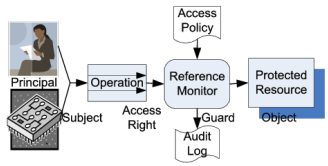
\includegraphics[width=0.75\linewidth]{chapters/2/images/rmm.png}
\end{figure}

Il \textbf{reference monitor} è un \textbf{sistema dotato di una politica di controllo 
degli accessi}. Si occupa di:
\begin{itemize}
    \item \textbf{autenticare chi vuole accedere}
    \item \textbf{autorizzare} o meno le operazioni richieste in base ai permessi 
    \item fare \textbf{audit} $\rightarrow$ tenere un log delle azioni compiute
\end{itemize}

\section{Definizioni}
\begin{itemize}
    \item La \textbf{sicurezza informatica} è l'insieme di strumenti, politiche, linee guida \dots che 
    possono essere utilizzate per proteggere l'ambiente e le risorse dell'organizzazione e 
    degli utenti del cyberspazio 
    \item I \textbf{beni dell'organizzazione e degli utenti} comprendono i dispositivi informatici 
    connessi, personale, infrastrutture e la totalità delle informazioni trasmesse e/o 
    archiviate nel cyberspazio 
    \item Gli \textbf{obiettivi} generali di sicurezza comprendono \textit{disponibilità, integrità e 
    confidenzialità}
    \item \textit{Sottoinsiemi} della sicurezza informatica:
    \begin{itemize} 
        \item \textbf{Sicurezza delle informazioni:} conservazione della CIA delle informazioni 
        \item \textbf{Sicurezza delle reti:} protezione delle reti e del loro servizio da modifiche non 
        autorizzate e garanzia che la rete svolga correttamente le sue funzioni critiche
    \end{itemize}
\end{itemize}

\section{Sfide della sicurezza informatica}

\begin{itemize}
    \item Non è semplice; può avere requisiti semplici ma \textbf{meccanismi di implementazione complessi}
    \item Nello sviluppo di un meccanismo di sicurezza, si deve sempre \textbf{considerare 
    potenziali attacchi}
    \item Le procedure utilizzate per fornire particolari servizi possono essere \textbf{controintuitive 
    poiché complesse}
    \item Bisogna decidere \textbf{dove utilizzare i meccanismi di sicurezza}, sia a livello 
    logico che a livello fisico
    \item I meccanismi di sicurezza in genere coinvolgono \textbf{più di un algoritmo 
    o protocollo}
    \item Una battaglia \textbf{continua} tra attaccante e difensore
\end{itemize}

\section{Principi fondamentali di progettazione della sicurezza}
\begin{itemize}
    \item \textbf{Fail-safe default:} nel caso in cui il sistema vada in default, deve rimanere
    in uno \textit{stato protetto}
    \item \textbf{Economia di meccanismo:} i meccanismi devono essere il più semplice possibile 
    \item \textbf{Mediazione completa:} \textit{tutti} gli accessi devono essere controllati per assicurarsi 
    che siano consentiti; solitamente accade che solo la prima interazione è controllata 
    \item \textbf{Design aperto:} la sicurezza non deve dipendere dalla segretezza della sua progettazione 
    o implementazione
    \item \textbf{Seperazione dei privilegi:} un sistema non dovrebbe concedere l'autorizzazione in base 
    a \textit{una singola} condizione
    \item \textbf{Minimi privilegi:} devono essere concessi il minor numero possibile di privilegi
    ad ogni soggetto; eventuali permessi addizionali devono essere concesso per il tempo minimo possibile
    \item \textbf{Accettabilità psicologica:} i meccanismi di sicurezza non dovrebbero rendere l'accesso 
    ad una risorsa più difficile
    \item \textbf{Isolamento}
    \item \textbf{Incapsulamento}
    \item \textbf{Modularità}
    \item \textbf{Stratificazione (\textit{layering})}
    \item \textbf{Minima sorpresa:} evitare che l'utente si trovi davanti a situazioni inaspettate 
    che potrebbero portarlo a seguire comportamenti scorretti
\end{itemize}

\section{Superificie di attacco}
Una superficie di attacco è costituita dalle \textbf{vulnerabilità raggiungibili e sfruttabili} in 
un sistema, come ad esempio:
\begin{itemize}
    \item porte aperte verso l'esterno
    \item interfacce web
    \item dipendente con accesso a dati sensibili 
    \item \dots
\end{itemize}
$\rightarrow$ è necessario \textbf{ridurre al minimo} la superificie di attacco

\subsection{Categorie di attacco}
\begin{itemize}
    \item Superificie di attacco di \textbf{rete}: sono incluse vulnerabilità del protocollo
    di rete, che possono portare a DoS, interruzione dei collegamenti di comunicazioni ed altri 
    attacchi intrusivi
    \item Superficie di attacco \textbf{software}: vulnerabilità nel codice delle applicazioni; un focus 
    particolare è il software per server web 
    \item Superificie di attacco \textbf{umano}: vulnerabilità create dal personale o da estranei, come 
    \textit{social engeneering}, errore umano o intrusi
\end{itemize}




























\chapter{Controllo degli accessi}

Il controllo degli accessi è un elemento centrale nella sicurezza 
informatica. È il \textbf{meccanismo} che definisce una \textbf{politica 
di sicurezza} per la quale si decide quali utenti possano accedere o 
meno ad una risorsa.

\noindent Si basa su tre principi fondamentali:
\begin{itemize}
    \item \textbf{Autenticazione:} verifica che le credenziali fornite 
    siano valide 
    \item \textbf{Autorizzazione:} concessione di un permesso ad un'entità
    affinché possa accedere ad una risorsa del sistema 
    \item \textbf{Auditing:} verifica delle attività e dei registri di 
    sistema
\end{itemize}

\begin{figure}[H]
    \centering
    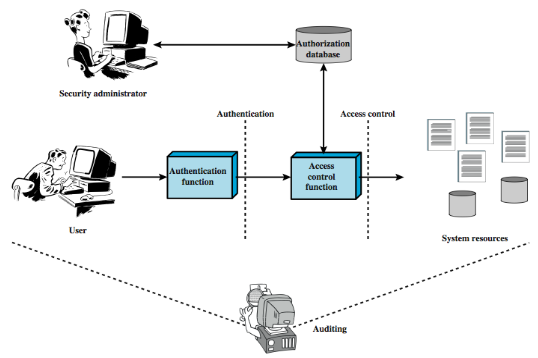
\includegraphics[width=1\linewidth]{chapters/3/images/ac.png}
\end{figure}

\section{Requisiti di sicurezza}

\subsection{Requisiti di sicurezza di base}
\begin{itemize}
    \item Limitare l'accesso al sistema informativo agli \textbf{utenti aurotizzati}, ai processi che agiscono 
    per conto degli utenti autorizzati o ai dispositivi 
    \item Limitare l'accesso al sistema informativo alle tipologie di funzioni che gli utenti 
    autorizzati possono eseguire 
\end{itemize}

\subsection{Requisiti di sicurezza derivati}
\begin{itemize}
    \item \textbf{separare i doveri} dei singoli individui per ridurre il rischio di attività malevole
    \item utilizzare \textbf{account non privilegiati} quando si accede a funzioni non di sicurezza 
    \item \textbf{impedire agli utenti non privilegiati} di eseguire funzioni privilegiate e controllare 
    l'esecuzione di tali funzioni 
    \item limitare i \textbf{tentativi di accesso} non riusciti 
    \item utilizzare il \textbf{blocco della sessione} per nascondere l'accesso ai dati dopo un periodo di inattività
    \item fornire \textbf{avvisi di privacy} e sicurezza secondo le norme vigenti 
    \item \textbf{terminare automaticamente} la sessione dopo una determinata azione 
    \item \textbf{monitorare e controllare} le sessioni di \textbf{accesso remoto}
    \item usare sistemi \textbf{crittografici} per garantire la riservatezza delle sessioni per accessi da remoto 
    \item \textbf{instradare l'accesso remoto} tramite punti di controllo degli accessi 
    \item \textbf{autorizzare} l'esecuzione remota di \textbf{comandi privilegiati}
    \item \textbf{autorizzare l'accesso wireless} prima di consentire tali connessioni
\end{itemize}

\section{Elementi di Access Control}
\begin{itemize}
    \item \textbf{Soggetto:} entità che può accedere agli oggetti (ad esempio, un processo che 
    rappresenta l'utente)
    \item \textbf{Oggetto:} risorsa ad accesso controllato (file, directory, \dots)
    \item \textbf{Diritto di accesso:} modo in cui un soggetto accede ad un oggetto (lettura, scrittura, \dots) 
\end{itemize}

\section{Politiche di controllo degli accessi}
\begin{itemize}
    \item \textbf{DAC:} controlla l'accesso in base all'identità del soggetto e alle autorizzazioni 
    che indicano che è/non è consentito fare ai richiedenti 
    \item \textbf{MAC:} controlla l'accesso in base al confronto tra delle specifiche etichette di sicurezza 
    applicate agli oggetti e le autorizzazioni di sicurezza 
    \item \textbf{RBAC:} controlla l'accesso in base al ruolo che l'utente ha nel sistema e alle regole 
    che stabiliscono quali accessi sono consentiti a quali ruoli 
    \item \textbf{ABAC:} controlla l'accesso in base agli attributi dell'utente
\end{itemize}

\subsection{DAC}
Il controllo dell'accesso viene fatto sull'\textbf{identità del soggetto richiedente} 
e delle \textbf{regole di accesso}. Definito \textit{discrezionale} perché un'entità potrebbe 
avere i privilegi di accessi che le permettono, a sua volta, di concedere l'accesso ad 
un'altra entità.

\noindent Si può rappresentare mediante una matrice di accesso, dove:
\begin{itemize}
    \item elenca i soggetti in una dimensione (colonne)
    \item elenca gli oggetti nell'altra dimensione (righe)
    \item ogni cella specifica i diritti di accesso di quel soggetto a quel determinato oggetto 
\end{itemize}

\begin{figure}[H]
    \centering
    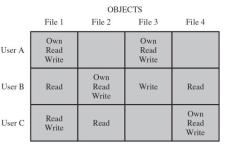
\includegraphics[width=0.8\linewidth]{chapters/3/images/dac-matrix.png}
\end{figure}

Questa matrice ha il problema di essere \textit{sparsa}, ovvero molto grande e 
con molte celle vuote

$\rightarrow$ viene trasformata in una serie di liste per risorse ed utenti

\begin{figure}[H]
    \centering
    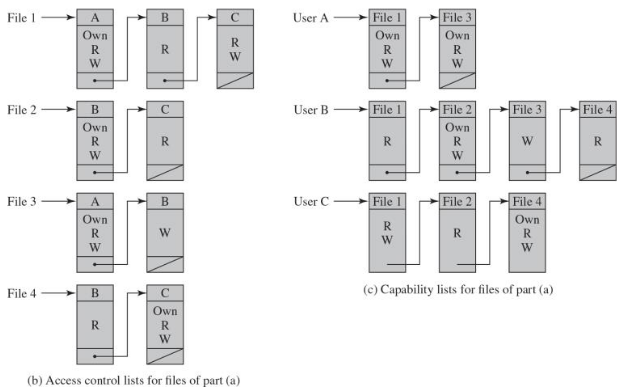
\includegraphics[width=1\linewidth]{chapters/3/images/dac-list.png}
\end{figure}


\subsection{MAC}
Controlla l'accesso in base al confronto tra:
\begin{itemize}
    \item \textbf{Etichette di sicurezza} che indicano quanto sono sensibili le risorse 
    \item \textbf{Autorizzazioni di sicurezza} che indicano quali entità del sistema 
    sono idonee ad accedere a quali risorse 
\end{itemize}

\noindent Questa politica è definita obbligatoria (\textit{mandatory}) perché un'entità che ha accesso 
ad una risorsa non può estendere il permesso ad un'altra; può farlo solo l'amministratore di sistema.

\noindent I sistemi MAC si dividono in:
\begin{itemize}
    \item \textbf{\textit{Multilevel security systems:}} consiste in una struttura verticale di 
    livelli di sicurezza; agli utenti viene assegnato un livello e possono accedere solo a risorse
    con livello uguale o inferiore 
    \item \textbf{\textit{Multilateral security systems:}} l'accesso viene assegnato in base a segmenti che formano 
    gruppi costituiti da livelli di sicurezza e parole in codice 

    $\rightarrow$ si ottiene una struttura orizzontale, che contiene livelli di sicurezza verticali aggiuntivi
\end{itemize}

\subsubsection{Vantaggi e svantaggi}
\begin{itemize}
    \item Il MAC è uno dei sistemi di accesso più sicuri, poiché è praticamente a prova di manomissione
    \begin{itemize}
        \item gli utenti non possono fare modifiche 
        \item il controllo è automatizzato 
        \item i dati non possono essere modificati senza apposita autorizzazione 
    \end{itemize}
    \item \dots tuttavia 
    \begin{itemize}
        \item richiede una pianificazione dettagliata e lavoro amministrativo
        \item controllare e aggiornare i diritti di accesso 
        \item manutenzione per aggiunta di nuovi dati o utenti e relative modifiche 
        \item $\rightarrow$ elevato carico di lavoro per l'amministratore
    \end{itemize}
\end{itemize}

\subsection{RBAC}
Ci sono quattro tipi di entità:
\begin{itemize}
    \item \textbf{Utente:} una persona che ha accesso al sistema; ogni individuo 
    ha un ID associato 
    \item \textbf{Ruolo:} inteso come una funziona lavorativa all'interno dell'organizzazione
    \item \textbf{Autorizzazione:} approvazione di una modalità di accesso ad uno o più oggetti 
    \item \textbf{Sessione:} mappatura tra un utente e un sottoinsieme dei ruoli a cui è assegnato
\end{itemize}

\begin{figure}[H]
    \centering
    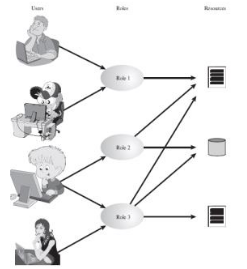
\includegraphics[width=0.7\linewidth]{chapters/3/images/rbac.png}
\end{figure}


\section{Unix security model}
In Linux ci sono tre entità da considerare:
\begin{itemize}
    \item \textbf{Soggetto:} può essere un utente o un processo 
    \item \textbf{Oggetto:} file, cartelle, \dots
    \item \textbf{Operazioni consentite:} lettura, scrittura, esecuzione 
\end{itemize}

\noindent In Unix, ogni utente ha associato un id univoco, detto \textbf{UID}; può appartenere a 
gruppi di utenti, anch'essi identificati da un id univoco detto \textbf{GID}. Tutti gli utenti 
appartenenti ad un gruppo possono condividere tra loro oggetti.

\noindent Ad ogni file è assegnato un unico utente proprietario e un unico gruppo proprietario. L'autorizzazione 
viene concessa mediante una ACL che identifica le operazioni che i soggetti possono fare.

\begin{figure}[H]
    \centering
    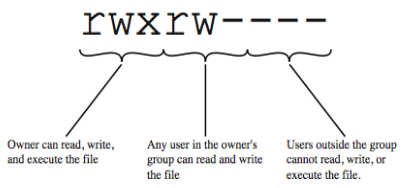
\includegraphics[width=0.7\linewidth]{chapters/3/images/unix-permessi.png}
\end{figure}

\subsection{Processi in Linux}
Ogni processo è isolato dagli altri e non possono accedere alla memoria altrui. Ogni processo viene 
eseguito con le autorizzazione dell'UID dell'utente che lo sta eseguendo. 

\noindent Nel momento della creazione, ad ogni processo sono assegnati tre ID (inizialmente tutti uguali 
all'UID):
\begin{itemize}
    \item \textbf{Effective UID:} determina le autorizzazioni per il processo 
    \item \textbf{Real UID:} determina l'utente che ha avviato il processo 
    \item \textbf{Saved UID:} EUID prima di eventuali modifiche
\end{itemize}

\noindent L'utente \textit{root} può cambiare EUID/RUID/SUID a valori arbitrari; utenti non privilegiati
possono cambiare EUID solo a RUID o SUID

\subsection{Unix file access control}
Le modifiche agli ID sono apportate mediante i comandi \textit{setUID} e \textit{setGID}; questa modifica 
permette ai programmi non privilegiati di accedere a risorse generalmente non accessibili.

\noindent Le directory possono aver impostato uno \textit{\textbf{sticky bit}}: specifica che solo il proprietario di un file nella cartella
può apportare una modifica a quel file 

\noindent Il \textit{\textbf{superuser}} è esente dalle consuete restrizioni di controllo degli accessi, ha 
accesso a tutto il sistema. 
\chapter{Politiche di sicurezza}

La \textit{gestione della sicurezza} è un \textit{processo formale} 
per rispondere alle domande:
\begin{itemize}
    \item quali sono i beni da proteggere
    \item quali sono le possibili minacce
    \item come si possono contrastare le minacce 
\end{itemize}

\noindent Questo processo ha natura iterativa, ed è contenuto nella ISO 31000; in 
questa norma viene descritto un \textit{modello per la gestione della sicurezza 
delle informazioni} che comprende le seguenti fasi:
\begin{itemize}
    \item \textbf{Plan:}
    \begin{itemize}
        \item stabilire politiche, processi e procedure di sicurezza
        \item eseguire la valutazione del rischio 
        \item sviluppare un piano di trattamento del rischio 
    \end{itemize}
    \item \textbf{Do:}
    \begin{itemize}
        \item implementare il piano di trattamento del rischio
    \end{itemize}
    \item \textbf{Check:}
    \begin{itemize}
        \item monitorare e mantenere il piano di trattamento del rischio
    \end{itemize}
    \item \textbf{Act:}
    \begin{itemize}
        \item mantenere e migliorare la gestione dei rischi 
        \item risposta ad incidenti, analisi di vulnerabilità e riprendere il ciclo iterativamente
    \end{itemize}
\end{itemize}

\newpage
\section{Definizioni}
\begin{itemize}
    \item \textbf{Rischio:} esprime la possibilità che un attacco causi danni ad una 
    organizzazione
    \item \textbf{Risorsa:} tutto ciò che necessita di essere protetto
    \begin{itemize}
        \item \textit{hw}
        \item \textit{sw}
        \item \textit{reputazione}
    \end{itemize}
    
    \noindent La valutazione di una risorsa viene fatta in base:
    \begin{itemize}
        \item ai costi da sostenere per sostituire la risorsa nel caso non sia più disponibile 
        \item perdita di incassi in caso di attacco 
    \end{itemize}
    \item \textbf{Vulnerabilità:} punti deboli che possono essere sfruttati per causare danni al 
    sistema; possono essere classificate come:
    \begin{itemize}
        \item critico 
        \item moderato 
        \item basso
    \end{itemize}
\end{itemize}












\chapter{Malware}

Una definizione \textit{informale} può essere quella di programma \textbf{malevolo}, solitamente 
inserito di nascosto in un sistema, che ha lo scopo di compremettere la riservatezza, l'integrità o 
la disponibilità del sistema stesso.


\noindent I malware sono classificati in base a:
\begin{itemize}
    \item \textbf{Propagazione} (sw, rete, social engeneering, \dots)
    \item \textbf{Azioni sui dati} colpiti (corruzione, furto, crittografia, \dots)
    \item \textbf{Attack kit} (strumenti già pronti per attaccare)
    \item \textbf{Attori e/o motivazioni} dell'attacco
\end{itemize}

\begin{figure}[H]
    \centering
    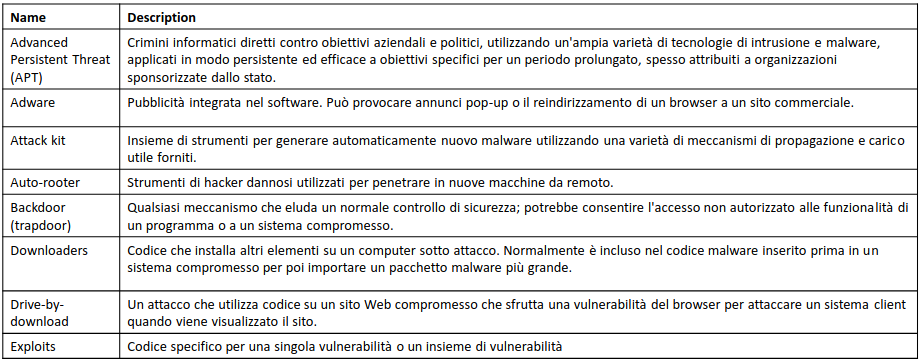
\includegraphics[width=1\linewidth]{chapters/5/images/classification1.png}
\end{figure}

\begin{figure}[H]
    \centering
    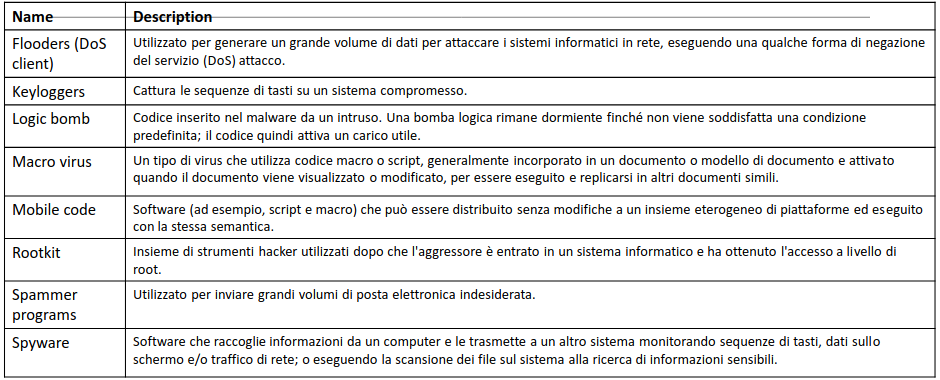
\includegraphics[width=1\linewidth]{chapters/5/images/classification2.png}
\end{figure}

\begin{figure}[H]
    \centering
    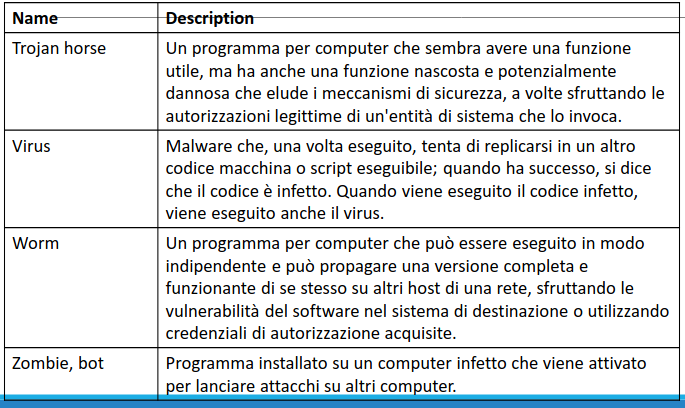
\includegraphics[width=1\linewidth]{chapters/5/images/classification3.png}
\end{figure}

\section{Trojan}
È un programma che ha un effetto evidente e atteso dall'utente, che ha però anche un 
effetto \textbf{nascosto} che viola le politiche di sicurezza e che viene condotto senza l'autorizzazione 
dell'utente

\section{Virus}
È un codice che può replicarsi modificando altri file o programmi per inserire codice in 
grado di replicarsi a sua volta; questa \textbf{proprietà di replicazione} è ciò distingue 
i virus dagli altri tipi di malware. Non svolge nessuna azione evidente, ma cerca di rimanere 
nell'ombra.

\noindent La replica richiede un certo tipo di assistenza da parte dell'utente, come ad esempio
cliccare su un allegato.

\noindent Un virus è composto da tre parti:
\begin{itemize}
    \item \textbf{Meccanismo di infezione}
    \item \textbf{Trigger:} evento che determina quando il payload viene attivato
    \item \textbf{Payload:} cosa fa il virus (oltre a diffondersi)
\end{itemize}

\noindent I virus attraversano quattro fasi:
\begin{enumerate}
    \item \textbf{Dormiente:} il virus è inattivo in attesa di essere attivato 
    \item \textbf{Scatenante:} il virus viene attivato 
    \item \textbf{Propagazione:} il virus inserisce una copia di sé stesso in certe parti del sistema; ogni programma 
    infetto conterrà ora un altro virus che entrerà a sua volta in fase di propagazione 
    \item \textbf{Esecutiva:} la funzione viene eseguita
\end{enumerate}

\subsection{Vettori di infezione}
I principali vettori di infezione sono:
\begin{itemize}
    \item \textbf{Boot sector} di dispositivi esterni; il codice è inserito nel boot sector e viene 
    eseguito in fase di avvio 
    \item \textbf{Eseguibili}
    \item \textbf{File macro:} il virus si attacca ai documenti per propagarsi 
\end{itemize}

\subsection{Classificazione dei virus}
È possibile classificare i virus in base alle \textbf{tecniche usate per superare i controlli 
di sistema:}
\begin{itemize}
    \item \textbf{Cifratura del virus:} crea una chiave per \textit{"crittografarsi"}; quando viene 
    chiamato un programma infetto, con tale chiave viene decifrato il virus. Per evitare pattern 
    di bit, durante la propagazione la chiave viene cambiata
    \item \textbf{Stealth virus:} si nasconde dal rilevamento da parte dell'antivirus, tramite mutazione 
    o compressione del codice 
    \item \textbf{Polymorphic virus:} durante la replica crea copie che svolgono la stessa funzione 
    ma che hanno pattern di bit diversi 
    \item \textbf{Metamorphic virus:} si riscrive completamente ad ogni iterazione per aumentare la 
    difficoltà di rilevamento
    \item \textbf{Compression virus:} comprimono il file eseguibile in modo che la versione infetta 
    abbia la stessa dimensione di quella originale
\end{itemize} 

\section{Worm}
I worm sono programmi \textit{stand alone} (a differenza dei virus che devono essere attivati 
da un qualche evento) in grado di replicarsi.

\noindent Le fasi di esecuzione sono:
\begin{itemize}
    \item \textbf{Probing:} cerca informazioni sulla macchina 
    \item \textbf{Expoloitation:} sfrutta le informazioni raccolte per trovare vulnerabilità
    \item \textbf{Replicazione}
    \item \textbf{Attacco} (payload)
\end{itemize}

\section{Drive-by-download}
Sfruttano \textbf{vulnerabilità del browser} per installare codice malevolo ad insaputa dell'utente 
nel momento in cui visita la pagina web dell'attaccante. 

\section{Clickjacking}
L'attaccante intercetta un \textit{click} dell'utente per costringerlo a fare delle cose 
contro la sua volontà.

\section{Zombie e botnet}
Lo \textit{zombie} è una singola macchina, mentre la \textit{botnet} è un insieme di macchine 
zombie controllate da una singola entità; vengono usate per fare DDoS, phishing, spamming, \dots

\section{Rootkit}
È un insieme di programmi installati su un sistema per mantenere l'accesso ad un sistema, ad 
esempio, con privilegi di amministratore, nascondendo le prove della sua presenza e aggirando 
i meccanismi di controllo.

\noindent Permettono di fare attacchi anche con scarse conoscenze tecniche.

\section{Scareware}
Software che hanno lo scopo di diffondere shock, ansia e/o la percezione di una minaccia; sono 
un attacco di \textit{social engeneering}.

\section{Ransomware}
Software che tiene in ostaggio il sistema per richiedere un riscatto all'utente, spesso tramite
cifratura.

\section{Vulnerabilità zero-day}
Si intende un'exploit non ancora nota e che non ha quindi una contromisura.

\section{Spear phishing}
Viene \textbf{studiato nel dettaglio il bersaglio}, in modo tale da fare del phishing più mirato 
ed efficace.

\section{Spyware}
Malware che raccoglie piccole informazioni alla volta sugli utenti a loro insaputa,
come ad esempio un \textit{keylogger}.

\section{APT - Advanced Persistent Threats}
\begin{itemize}
    \item \textit{\textbf{Advanced:}} è un'applicazione con un ampia varietà di tecnologie di intrusione e malware
    \item \textit{\textbf{Persistent:}}
    attacchi per un periodo di tempo prolungato verso il target
    \item \textit{\textbf{Target:}} target selezionati in modo accurato
\end{itemize}

\noindent Le fasi principali di un attacco tramite APT sono:
\begin{itemize}
    \item \textbf{Ricognizione:} si sceglie una vittima e la si studia 
    \item \textbf{Weaponization:} si mette un trojan che permette accesso remoto in un payload consegnabile (email, USB, web)
    \item \textbf{Sfruttamento:} il codice malevolo viene attivato per portare a termine il suo scopo
\end{itemize}


\newpage
\section{Approcci alle contromisure per i malware}
Le principali contromisure da adottare sono:
\begin{itemize}
    \item assicurare di \textbf{aggiornare} tutti i sistemi
    \item ridurre al \textbf{minimo le vulnerabilità}
    \item impostare adeguati \textbf{controlli} di accesso alle applicazioni e ai dati 
    \item \textbf{limitare} il numero di file a cui un utente può accedere, e che quindi può 
    potenzialmente infettare
\end{itemize}

\noindent Le azioni da prendere nel caso il sistema venga attaccato sono:
\begin{itemize}
    \item \textbf{Rilevamento:} accertarsi della presenza del virus; può essere fatto con:
    \begin{itemize}
        \item programmi anti-virus, 4 generazioni:
        \begin{itemize}
            \item \textbf{scanner semplici} $\rightarrow$ ricercano malware noti 
            \item \textbf{scanner euristici} $\rightarrow$ utilizzano regole euristiche
            \item \textbf{trap di attività:} viene cercato il malware in base alle sue azioni piuttosto che in base alla sua 
            struttura $\rightarrow$ l'analisi è dinamica 
            \item \textbf{protezione completa:} più tecniche usate insieme 
        \end{itemize}
        \item meccanismi di protezione perimetrale nei firewall
    \end{itemize}
    \item \textbf{Identificazione:} individuare lo specifico malware
    \item \textbf{Rimozione} di tutte le tracce dal sistema
\end{itemize}










\chapter{Autenticazione}
Processo per determinare se un utente, un'applicazione o un processo che agisce per conto di un utente 
\textbf{è effettivamente chi o cosa dichiara di essere}; si fa un confronto tra le credenziali 
inserite e quelle memorizzate nel sistema.

\section{Principi di autenticazione}
\begin{itemize}
    \item \textbf{Identità digitale:} è la rappresentazione unica di un soggetto, consiste in 
    un attributo o un insieme di attributi che descrivono univocamente un soggetto 
    \item \textbf{Prova dell'identità:} stabilisce che un soggetto è chi afferma di essere ad un determinato 
    livello di certezza
    \item \textbf{Autenticazione digitale:} il processo di determinazione della validità di uno o più 
    autenticatori utilizzati per rivendicare un'identità digitale 
\end{itemize}

\section{Requisiti di sicurezza}
\begin{itemize}
    \item \textbf{Di base:} 
    \begin{itemize}
        \item \textbf{identificare} gli utenti del sistema informativo e i processi che agiscono per loro conto 
        \item autenticare (o \textbf{verificare}) le identità di tali utenti 
    \end{itemize} 
    \item \textbf{Derivati:}
    \begin{itemize}
        \item utilizzare l'\textbf{autenticazione a più fattori}
        \item impiegare meccanismi resistenti ad \textbf{attacchi di replay}
        \item impedire il riutilizzo degli \textit{id} per un certo intervallo di tempo 
        \item disabilitare gli \textit{id} dopo un periodo di inattività
        \item applicare una \textbf{complessità minima} della password
        \item proibire il \textbf{riutilizzo} delle password 
        \item memorizzare e trasmettere solo password \textbf{criptate}
        \item \textbf{oscurare il feedback} delle informazioni di autenticazione
    \end{itemize}
\end{itemize}

\section{Metodi di autenticazione}
\begin{itemize}
    \item \textbf{qualcosa che uno sa:} password, \dots
    \item \textbf{qualcosa che uno ha:} token $\rightarrow$ smartcard, chiave fisica, \dots
    \item \textbf{qualcosa che l'individuo è:} tratto biometrico
    \item \textbf{qualcosa che l'individuo fa:} biometria dinamica
\end{itemize}

\section{Password}
Lo schema standard \textit{id-password} è soggetto a diverse vulnerabilità:
\begin{itemize}
    \item canale tra client e server 
    \item compromissione del client 
    \item compromissione del server 
    \item social engeneering 
    \item password deboli 
\end{itemize}

\noindent Esistono diversi tipi di attacco alle password:
\begin{itemize}
    \item attacchi a \textbf{dizionario} 
    \item \textbf{forza bruta}
    \item uso della \textbf{stessa password} per più servizi
\end{itemize}

\subsection{Memorizzazione delle password}
Nello vecchio sistema UNIX veniva memorizzato nel file \texttt{/etc/passwd} l'hash delle password 
insieme al suo id.

\noindent Oggi, la password viene salvata come \textbf{hash} nel file \textbf{\texttt{/etc/shadow}},
che è \textbf{leggibile solo da \textit{root}}.

\noindent Per proteggersi da attacchi di forza bruta, è possibile usare un \textbf{salt}: invece che memorizzare 
l'hash della password, ad esso viene concatenato all'inizio e/o alla fine un \textit{numero casuale} di 
lunghezza arbitraria; vengono usati salt fino a 48 bit.

\subsection{Cracking delle password}
\begin{itemize}
    \item attacchi di dizionario 
    \item tabelle \textit{rainbow}: contengono hash precalcolati di diversi dizionari, con già inseriti 
    dei salt 
\end{itemize}

\noindent La maggioranza degli attacchi \textbf{sfrutta password deboli}; la soluzione è costringere 
gli utenti ad usare \textbf{password complesse}.

\subsection{Utilizzo delle password su canali non sicuri}
Esistono tre approcci:
\begin{itemize}
    \item \textbf{One-time-password}
    \item \textbf{Challenge response:} chi si autentica dimostra di conoscere un segreto (challenge); 
    di norma vengono usati anche timestamp per evitare attacchi di replay
    \item \textbf{Zero knowledge proof:} chi si autentica fornisce una prova di conoscere la password 
    senza fornirla esplicitamente 
\end{itemize}

\section{Altri metodi di autenticazione}
\begin{itemize}
    \item \textbf{Smart token:} dispositivi dotati di \textbf{capacità computazionale}, possono fare diversi tipi di controlli 
    \item \textbf{Smart card:} forniscono informazioni una volta inserite nel sensore, non hanno sistemi di calcolo 
    \item \textbf{Autenticazione biometrica}
    \item \textbf{Autenticazione reciproca:} permettono ad entrambe le parti di accertarsi reciprocamente della propria identità
\end{itemize}


\section{Problemi di sicurezza dell'autenticazione}
\begin{itemize}
    \item \textbf{Intercettazione}, ad esempio con un attacco che implica la vicinanza fisica di utente ed attaccante
    \item \textbf{Attacchi host:} diretti al file dell'utente in cui sono contenute le password/token/\dots
    \item \textbf{Replay:} l'avversario ripete una risposta dell'utente acquisita in precedenza, senza che il server 
    sia in grado di distinguerla; si può contrastare con tre approcci:
    \begin{itemize}
        \item allegare un \textbf{numero di sequenza} a ciascun messaggio
        \item \textbf{timestamp} per verificare la validità
        \item \textbf{challenge-response:} quando una parte invia un messaggio, deve contenere il
        \textit{nonce} del messaggio precedente
    \end{itemize}
    \item \textbf{Attacchi client:} l'avversario cerca di autenticarsi senza accedere all'host remoto 
    \item \textbf{DoS:} tenta di disabilitare un servizio 
\end{itemize}







\chapter{Modello ISO-OSI}
Ad oggi internet è il più grande sistema ingegneristico mai creato dall'umanità, che 
comprende miliardi di utenti e macchine.

\noindent Le operazioni chiave nella rete sono:
\begin{itemize}
    \item invio e consegna di pacchetti 
    \item instradamento dei pacchetti 
    \item individuazione degli indirizzi
\end{itemize}

\section{Protocolli}
Sono un \textbf{insieme formale di regole} durante un'interazione; descrivono come i computer trasmettono 
i dati attraverso una rete, come il formato e l'ordine dei messaggi, oltre alle azioni intraprese sulla 
trasmissione e/o ricezione di essi.

\section{Layering}
Per far fronte alla complessità, i protocolli sono organizzati in uno \textit{stack} di livelli

$\rightarrow$ i dati vengono passati dal livello più alto a quello più basso 

\noindent Questo facilita la manutenzione e l'aggiornamento del sistema.

\begin{figure}[H]
    \centering
    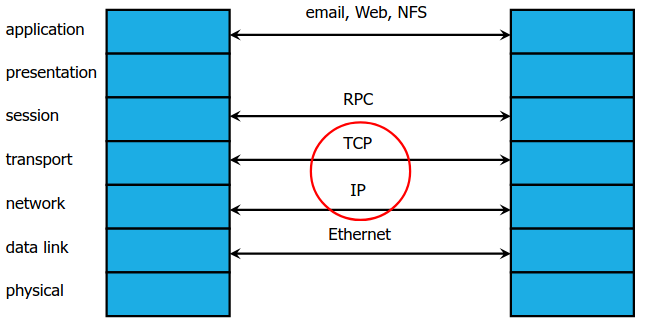
\includegraphics[width=1\linewidth]{chapters/7/images/osi-stack.png}
    \caption{OSI stack}
\end{figure}

\section{Principio end-to-end}
Le funzionalità specifiche dell'applicazione risiedono nei nodi finali di comunicazioni della rete, 
piuttostoc che nei nodi intermedi come \textit{gateway} e \textit{router}; l'\textit{intelligenza}
sta ai vertici della rete.

\section{Tipi di indirizzi in Internet}

\begin{itemize}
    \item \textbf{MAC} nel livello di accesso alla rete 
    \begin{itemize}
        \item associata alla scheda con interfaccia di rete 
        \item 48/64 bit 
    \end{itemize}
    \item \textbf{IP} per il livello di rete 
    \begin{itemize}
        \item 32bit per IPv4, 64bit per IPv6
        \item Ad esempio, 128.3.23.3
    \end{itemize}
    \item \textbf{IP + porte} per il livello di trasporto
    \begin{itemize}
        \item Ad esempio, 128.3.23.3:80
    \end{itemize}
    \item \textbf{Dominio} per livello di applicazione/umano 
    \begin{itemize}
        \item Ad esempio, www.inter.it 
    \end{itemize}
\end{itemize}

\subsection{Routing e traduzione degli indirizzi}
\begin{itemize}
    \item Routing tra indirizzi IP ed indirizzi MAC 
    \begin{itemize}
        \item protocollo di risoluzione degli indirizzi (ARP) per IPv4 
        \item Neighbour Discovery Protocol (NDP) per IPv6
    \end{itemize}
    \item Routing con indirizzi IP 
    \begin{itemize}
        \item TCP, UDP, IP per instradare pacchetti 
        \item Border Gateway Protocol per gli aggiornamenti delle tabelle di routing 
    \end{itemize}
    \item Traduzione da indirizzi IP a nomi di dominio 
    \begin{itemize}
        \item DNS
    \end{itemize}
\end{itemize}

\section{Interfaccia di rete}
Un computer può avere più interfaccie di rete; i pacchetti vengono trasmessi tra le interfacce 
di rete.



\noindent Impara l'indirizzo MAC di ogni computer ad esso connesso ed inoltra i frame solo al 
computer di destinazione.

\section{Netmask}
La netmask è una sequenza di 32 bit che identifica quali bit sono comuni negli indirizzi IP 
all'interno di una LAN (sottorete).

Ad esempio, 159.132.30.0/24 $\rightarrow$ 24 bit per la sottorete

\section{Tipi di minacce nella rete}
\begin{itemize}
    \item Confidenzialità (\textit{packet sniffing})
    \item Integrità (\textit{session hijacking})
    \item Disponibilità (DoS)
    \item \textit{Translation poisoning, routing}
\end{itemize}

\newpage
\section{ARP (Address Resolution Protocol)}
Il protocollo ARP connette il livello di rete con il livello dati, \textbf{convertendo un 
indirizzo IP in un indirizzo MAC}.

\noindent Ogni nodo mantiene una tabella (\textit{ARP cache}) in cui ci sono le associazioni 
già note; altrimenti, si chiede a tutti i nodi della rete locale chi ha un certo indirizzo IP.

$\rightarrow$ ARP funziona inviando $n$ messaggi broadcast e memorizzando nella cache le risposte, per utilizzi futuri:
\begin{itemize}
    \item \textit{ARP request} (effettuata in broadcast)
    \begin{itemize}
        \item \texttt{who has <IP1> tell <IP2>} 
    \end{itemize}
    \item \textit{ARP reply}
    \begin{itemize}
        \item \texttt{<IP1> is <MAC>}
    \end{itemize}
\end{itemize}

\subsection{ARP spoofing - Cache poisoning}
Viene fatta una \textit{assunzione di trust} nella LAN, dato che:
\begin{itemize}
    \item le richieste non vengono tracciate 
    \item gli annunci non sono autenticati 
    \item le macchine si fidano una dell'altra 
\end{itemize}

$\rightarrow$ una macchina malevola puà ingannare le altre 

\noindent Dato che una \textit{cache ARP} si aggiorna ogni volta che riceve una risposta ARP anche 
se non ha inviato alcuna richiesta \dots è possibile \textit{avvelenare} una cache inviando delle 
risposte \textit{"gratuite"}!

\section{MAC address e spoofing}
Le schede di rete sono indentificate da un numero seriale, che viene utilizzato come 
indirizzo all'interno della LAN.

\noindent Con i privilegi adeguati, è quasi sempre possibile (e facile) cambiare il numero 
MAC usato nella produzione dei frame

$\rightarrow$ conoscendo il MAC di una macchina assente, è immediato impersonarla

\newpage
\section{MAC address flooding}
\subsubsection{Switch}
Uno switch è un dispositivo che opera a livello di collegamento (link); ha più porte, ciascuna 
collegata ad un computer.
\noindent Quando i frame arrivano sulle porte dello switch, gli indirizzi MAC di orgine vengono 
appresi dall'intestazione del pacchetto e registrati in una tabella.
\begin{itemize}
    \item Se lo switch conosce già l'indirizzo MAC, inoltra il frame alla porta dell'indirizzo MAC 
    \item Se non esiste, lo switch funge da hub e inoltra il frame su ogni altra porta dello switch, mentre 
    memorizza il MAC per la prossima volta
\end{itemize}

\subsubsection{Attacco}
\noindent L'attacco di flooding viene spesso chiamato anche come attacco di overflow della 
tabella degli indirizzi MAC, dato che ha dimensioni limitate.

\noindent Il MAC flooding \textbf{invia un intero gruppo di indirizzi MAC di origine falsi}, fino 
a quando la tabella è satura e non può più salvare l'indirizzo MAC

$\rightarrow$ lo switch comincerà a trasmettere tutti i pacchetti ricevuti a tutte le altre macchine 
sulla rete 

\noindent I tool di attacco generano circa 160.000 voci MAC al minuto.


\chapter{Attacchi TCP/IP}

\section{Livello di trasporto}
La responsabilità principale del livello di trasporto è la consegna 
dei dati da processo a processo. I singoli processi in esecuzione su un 
dato host sono identificati dai loro numeri di porta.

\begin{figure}[H]
    \centering
    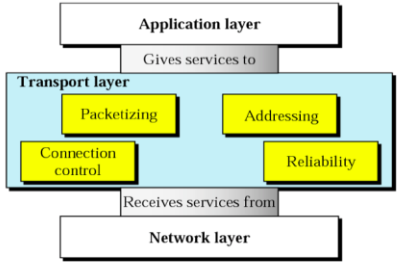
\includegraphics[width=0.7\linewidth]{chapters/8/images/trasporto.png}
\end{figure}

\noindent I due protocolli del livello di trasporto utilizzati in internet 
sono TCP e UDP.

\subsection{Porte}
Un numero di porta è un intero a 16 bit che assume un valore comprso 
tra 0 e 65535. I numeri di porta tra 0 e 1023 (i cosidetti \textit{numeri di
porta noti}) sono riservati ad applicazioni come HTTP, \dots

\section{TCP (Transmission Control Protocol)}
\begin{itemize}
    \item \textbf{Mittente:} suddivide i dati in pacchetti; ad ogni pacchetto è associato un numero di sequenza
    \item \textbf{Ricevitore:} riassembla i pacchetti nell'ordine corretto; i pacchetti persi vengono rispediti
\end{itemize}

\begin{figure}[H]
    \centering
    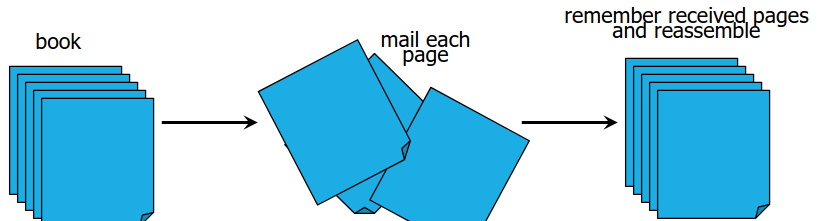
\includegraphics[width=1\linewidth]{chapters/8/images/tcp.png}
\end{figure}

\subsection{Flag TCP}
\begin{itemize}
    \item \textbf{SYN:} richiesta di connessione, primo pacchetto della comunicazione 
    \item \textbf{FIN:} intenzione del mittente di terminare la sessione
    \item \textbf{ACK:} conferma del pacchetto precedente
    \item \textbf{RST:} reset della sessione 
    \item \textbf{URG:} dati urgenti che vengono inviati con precedenza sugli altri (es. CTRL+C) 
\end{itemize}

\subsection{TCP handshake}
Le connessioni TCP vengono stabilite tramite un handshake a tre vie:
\begin{itemize}
    \item il server ha generalmente un listener passivo, in attesa di una richiesta di connessione 
    \item il client richiede una connessione inviando un pacchetto SYN 
    \item il server risponde inviando un pacchetto SYN/ACK, indicando un riconoscimento per la connessione 
    \item il client risponde inviando un ACK al server, stabilendo così la connessione
\end{itemize}

\begin{figure}[H]
    \centering
    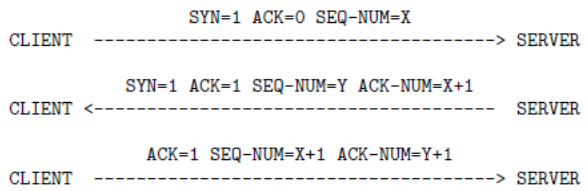
\includegraphics[width=0.8\linewidth]{chapters/8/images/tcp-handshake.png}
\end{figure}

\subsection{Problemi intrinsechi}
\begin{itemize}
    \item \textbf{Non c'è autenticazione} fra le parti; un utente malevolo potrebbe 
    intromettersi nella connessione fintanto che usa un \textit{sequence number} corretto 
    e gli indirizzi IP sono corretti 
    \item i \textbf{controlli di integrità} sono banali
\end{itemize}

\section{Spoofing}

\subsection{TCP spoofing}
Ogni connessione TCP ha uno stato associato:
\begin{itemize}
    \item numero di sequenza 
    \item numero di porta 
\end{itemize}

$\rightarrow$ è facile da indovinare, dato che si usano numeri di porta standard e numeri 
di sequenza prevedibili

\noindent È dunque possibile iniettare pacchetti in connessioni esistenti:
\begin{itemize}
    \item se l'attaccante conosce il numero di sequenza iniziale e la quantità di traffico, può indovinare 
    il probabile numero corrente 
    \item altrimenti, dato che la maggior parte dei sistemi accetta grandi finestre di numeri di sequenza per gestire 
    le perdite di pacchetti, invia un flusso di pacchetti con probabili numeri di sequenza
\end{itemize}

\subsection{IP spoofing}
Le autenticazioni locali su indirizzi IP sono insicure, specialmente 
all'interno di rete locali; l'header IP è falsificabile senza particolari 
difficoltà.
\begin{itemize}
    \item \textbf{Blind spoofing}
    
    \noindent Attacca da qualsiasi fonte; cerca di impersonare un host qualunque
    di internet, non facente parte della sottorete in cui si trova.
    
    \noindent \textit{Blind} perché l'attaccante non ha nessuna possibilità di vedere i 
    pacchetti mandati in risposta ai pacchetti \textit{"spoofati"} che ha spedito;
    questi ultimi saranno infatti spediti al vero host che l'attaccante sta impersonando, 
    impedendogli quindi di venire a conoscenza di \textit{ack number} e \textit{sequence number}
    corretti per continuare la connessione.

    \item \textbf{Non-blind spoofing}
    
    \noindent L'attaccante si trova nella stessa rete della vittima, quindi sarà in grado 
    di intercettare i pacchetti in risposta a quelli fraudolenti che ha inviato (tramite sniffer), e quindi 
    di ottenere il sequence number corretto.
\end{itemize}

\noindent I passaggi di IP spoofing sono:
\begin{enumerate}
    \item viene \textbf{scelta una vittima} e cercato un host considerato come fidato dalla vittima 
    \item si \textbf{disabilita l'host fidato} (ad esempio tramite SYN flooding)
    \item a questo punto si \textbf{contatta la vittima} e si ottiene un numero di sequenza valido, per provare 
    a predire il prossimo numero di sequenza 
    \item l'attaccante manda un pacchetto SYN utilizzando come IP mittente quello della macchina fidata. Anche se 
    l'hacker non riceve il SYN/ACK, può sempre rispondere in modo che la vittima pensi di aver stabilito correttamente la 
    connessione 
\end{enumerate}

\noindent La disabilitazione dell'host fidato è parte fondamentale, in quanto alla ricezione 
del pacchetto SYN/ACK potrebbe interrompere la connessione tramite un pacchetto RST.


\section{TCP session hijacking}

L'obiettivo è aprire una connessione con il server \textbf{impersonando la vittima}; 

\begin{itemize}
    \item L'attaccante apre una connessione autentica con il suo bersaglio (B), ricevendo un numero di sequenza 
    \item L'attaccante (C) si spaccia per il client (A)
    \begin{itemize}
        \item invia un pacchetto con l'indirizzo del client (A) nel campo dell'indirizzo sorgente
        e un numero di sequenza coerente con ciò che B si aspetta
    \end{itemize}
    \item Se l'attaccante indovina il numero di sequenza, il server presume di avere una connessione con A 
    \begin{itemize}
        \item L'attaccante non può vedere l'output di questa sessione, ma potrebbe eseguire comandi con i privilegi 
        di A sul server
    \end{itemize}
\end{itemize}

\begin{figure}[H]
    \centering
    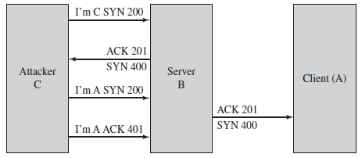
\includegraphics[width=0.8\linewidth]{chapters/8/images/tcp-hijack.png}
\end{figure}


\section{ACK storm}
Gli attacchi ACK storm si basano sul fatto che, quando si riceve un pacchetto con ACK più 
grande di quello inviato dal client ricevente, il client deve inviare l'ultimo pacchetto 
inviato all'altro lato e scartare il pacchetto ricevuto.

\noindent L'attacco prevede di:
\begin{itemize}
    \item prelevare un pacchetto da una connessione TCP tra un client e un server 
    \item generare due pacchetti, ciascuno inviato a una parte con l'indirizzo IP dell'altra
    \item inviare i pacchetti contemporaneamente
\end{itemize}

$\rightarrow$ la connessione entra in un ciclo infinito di ACK.

\noindent Come contromisura a questo attacco, si è modificato il protocollo facendo in modo che 
il pacchetto viene scartato senza dover rimandare la risposta.

\section{Attacco DoS}
Lo scopo è quello di impedire alla vittima di rispondere alle richieste; esistono 
due tipi di DoS:
\begin{itemize}
    \item \textbf{DoS bug:} sfrutta difetti di progettazione della vittima 
    \item \textbf{DoS flood:} vengono sfruttate delle bot-net per inondare di richieste la vittima
    \begin{itemize}
        \item un modo è quello di usare \textbf{ACK reflection attack:}
        
        \noindent L'attaccante invia del traffico con l'indirizzo IP della vittima ad un server intermedio (detto \textit{reflector}),
        che si occuperà di mandare le risposte alla vittima 

        $\rightarrow$ si può mandare una serie di SYN al reflector che inonderà la vittima di 
        SYN/ACK; la vittima vedrà l'IP del reflector e non quello dell'attaccante
    \end{itemize}
\end{itemize}

\subsection{SYN flood}
Prevede che l'attaccante \textbf{continui ad inviare richieste SYN al server} senza poi 
rispondere ai SYN/ACK ricevuti in risposta; in questo modo, il server dovrà dedicare risorse per rispondere 
ed attendere inutilmente che le connessione TCP aperte terminino l'handshake. L'idea è quella
di impedire al server di poter rispondere ad ulteriori richieste di connessione legittime.

\subsection{Contromisure ad attacco DoS}
Ci sono quattro approcci principali:
\begin{itemize}
    \item \textbf{aumentare le dimensioni del \textit{backlog}} (coda in cui il server memorizza le connessioni 
    iniziate che non hanno ancora terminato l'handshake)
    \item ridurre il \textbf{SYN-Received timer}, ovvero il tempo per cui una connesisone rimane nel backlog prima 
    che venga scartata 
    \item \textbf{SYN cookies:} il server inserisce le informazioni che di norma si salverebbero nel backlog 
    all'interno di un cookie che viene inserito nella risposta SYN/ACK inviata al client. Solo nel 
    momento in cui in server riceve risposta allora aprirà la connessione e le dedicherà risorse.

    \noindent Il cookie deve essere firmato e non modificabile; viene calcolato nel seguente modo 
    \begin{itemize}
        \item i primi \textbf{5 bit} sono dati da $t mod 32$, con $t$ \textbf{timestamp}
        \item i seguenti \textbf{3 bit} sono la codifica del numero di entry che il server avrebbe salvato nel backlog 
        \item gli ultimi \textbf{24 bit} sono il risultato di una funzione di hash, che prende in input:
        \begin{itemize}
            \item input IP server
            \item IP client
            \item porta del server
            \item porta client
            \item timestamp
        \end{itemize}
    \end{itemize}

    \noindent Nel momento in cui il client manda l'ACK in risposta con allegato il cookie, la \textbf{verifica}
        ha i seguenti passi:
        \begin{enumerate}
            \item viene verificato il timestamp per vedere se il pacchetto sia ancora valido 
            \item vien ricomputata la funzione di hash per vedere se il SYN sia ancora valido 
            \item vengono decodificati i 3 bit corrispondenti alla entry della coda di backlog
        \end{enumerate}
    \item \textbf{cancellazione di una entry a caso} per far posto a una nuova 
    \item uso di un \textbf{prolexic proxy:} si mette un proxy tra server e client; sarà il proxy a gestire 
    l'handshake, ed inoltrerà al server solo le richieste SYN di cui si riceve anche un ACK
\end{itemize}

\section{UDP (User Datagram Protocol)}














\chapter{Network e Port Scanning}
Dal punto di vista dell'\textbf{amministratore} di rete, la scansione è 
un'\textbf{attività preliminare fondamentale} per conoscere quali dispositivi siano 
collegati e configurazione abbiano; l'amministratore può conoscere come sia composto 
il sistema informatico da difendere.

\noindent Dal punto di vista dell'\textbf{attaccante}, accedere a queste informazioni 
permette di sapere a quali \textbf{vulnerabilità} sia esposta la rete (sistemi operativi 
in uso, sw non aggiornato, porte aperte sfruttabili, \dots).

\begin{figure}[H]
    \centering
    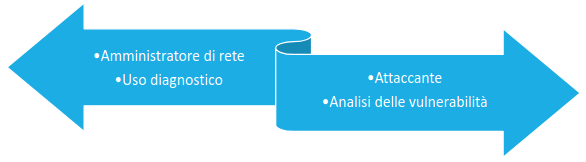
\includegraphics[width=0.9\linewidth]{chapters/9/images/intro.png}
\end{figure}

Le \textbf{attività principali} portate avanti dall'attaccante sono:
\begin{itemize}
    \item la \textbf{mappatura della rete} (network scanning, vedo quali macchine sono attive sulla rete)
    \item riconoscere i servizi UDP e TCP \textbf{disponibili} (port scanning)
    \item riconoscere i \textit{sistemi di filtraggio} usati per l'utente 
    \item determinare i \textit{sistemi operativi} usati 
\end{itemize}

\noindent Sia \textit{network scanning} che \textit{port scanning} sono rilevabili e sono \textbf{illegali}
(salvo autorizzazione del proprietario della rete/macchina).

\noindent Generalmente, salvo alcuni servizi che devono essere esposti verso 
l'esterno (come HTTP/HTTPS nel caso di un server web), il firewall blocca 
questo tipo di richieste.

\section{Tipologie di scansione}
Le scansioni vengono classificate in base al modo in cui sono compiute, al loro scopo e 
al numero di host coinvolti.

\subsection{Numero di host coinvolti}
\begin{itemize}
    \item un singolo host interroga diverse macchine 
    \item tanti host fanno scanning di una sola macchina (si cerca di lasciare meno tracce)
    \item tante macchine fanno scanning di tanti host 
\end{itemize}

\begin{figure}[H]
    \centering
    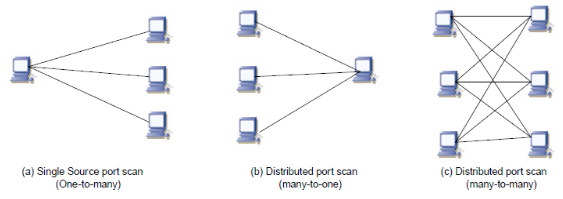
\includegraphics[width=0.9\linewidth]{chapters/9/images/tipi-scansioni.png}
\end{figure}

\subsection{Natura della scansione}
È possibile parlare di scanning:
\begin{itemize}
    \item \textbf{verticale:} più porte di una singola macchina vengono scansionate 
    \item \textbf{Orizzontale:} la stessa porta di più macchine viene controllata 
    \item \textbf{Ibrido:} combinazione delle precedenti
\end{itemize}


\noindent Per quanto riguarda la \textbf{natura della scansione}, 
si può classificare in:
\begin{itemize}
    \item \textbf{Scanning attivo:} si mandano pacchetti alla macchina da scansionare, che 
    possono essere generici o relativi a un particolare protocollo o sw 
    \item \textbf{Scanning passivo:} ci si limita a fare sniffing sulla rete e dedurre come sia 
    configurata la macchina
\end{itemize}

\begin{figure}[H]
    \centering
    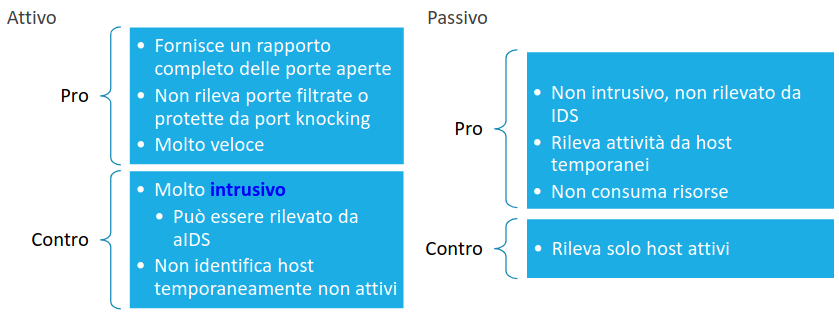
\includegraphics[width=1\linewidth]{chapters/9/images/attivo-passivo.png}
\end{figure}

\subsection{Scopo}
\begin{itemize}
    \item Si parla di \textbf{\textit{wide range scanning}} quando si analizza un 
    dato insieme di indirizzi 
    \item Si parla di \textbf{\textit{target-specific scanning}} quando la scansione 
    riguarda un'entità specifica
\end{itemize}

\section{Risultati (port scanning)}
I risultati di uno scan su una porta possono portare alle seguenti considerazioni:
\begin{itemize}
    \item \textbf{Aperta:} il target ha risposto, indicando che un servizio è in ascolto 
    su quella porta (\textit{connection accepted})
    \item \textbf{Chiusa:} il target ha risposto rifiutando la connessione (\textit{connection denied})
    \item \textbf{Bloccata/Filtrata:} un sistema di sicurezza perimetrale (come un firewall) ha 
    bloccato l'accesso alla porta, impedendo di individuare uno stato (\textit{connection dropped/filtered})
\end{itemize}

\section{Attacchi tramite protocolli noti}
\begin{itemize}
    \item \textbf{ARP scan:} tramite il protocollo ARP è possibile scoprire tutti i dispostivi 
    attivi su una rete locale; l'attacco consiste nel mandare una serie di richieste ARP in broadcast al fine 
    di collezionare tutti gli IP 
    \item \textbf{ICMP:} vengono mandati una serie di pacchetti ICMP \textit{echo request} (ping) per 
    poi rimanere in attesa della risposta (ICMP \textit{echo reply}); spesso questo approccio non è percorribile 
    in quanto i ping vengono spesso bloccati dagli amministratori di rete.

    \noindent Per aggirare questa contromisura, è possibile usare ICMP \textit{timestamp}
    \newpage
    \item \textbf{TCP:} sono possibili due approcci che sfruttano questo protocollo:
    \begin{itemize}
        \item \textbf{TCP SYN ping:} si manda un TCP SYN; nel caso in cui si riceve risposta SYN-ACK, 
        il servizio è attivo su quella porta 
        \item \textbf{TCP ACK ping:} si manda un pacchetto ACK; nel caso in cui si riceve risposta 
        RST, il servizio è attivo su quella porta 
    \end{itemize}
    \item \textbf{UDP ping:} si manda un pacchetto UDP vuoto; se l'host risponde, sappiamo che è attivo 
    su quella porta 
    \item \textbf{IP ping:} si mandano pacchetti con protocolli non abilitati (nell'header IP è prevista l'indicazione del protocollo) e 
    si verifica se l'host risponde (analogo a UDP ping)
\end{itemize}

\subsection{TCP connect scan}
È un attacco che fa uso della \textit{syscall} \texttt{connect()} per connettersi ad una 
socket esposta sulla rete in stato di listen.

\subsubsection{Open scan}
Le risposte ad un SYN possono essere:
\begin{itemize}
    \item SYN-ACK: porta aperta 
    \item RST: porta chiusa 
    \item \textit{nessuna rispsota} : porta filtrata da firewall
    \item ICMP unreachable: porta filtrata da un firewall
\end{itemize}

\subsubsection{Half-open scan}
Nel caso in cui si riceva un SYN-ACK, si restituisce un RST per \textbf{terminare la connessione}
TCP rimasta aperta.

\noindent Questo approccio è meno intruviso e quindi meno rilevabile.

\subsection{Stealth scan}
Gli attacchi di \textit{stealth scan} possono essere fatti in vari modi:
\begin{itemize}
    \item \textbf{SYN-ACK scan:} le richieste SYN sono spesso individuate e filtrate; si può invece 
    mandare un pacchetto SYN-ACK e dedurre informazioni dalla risposta
    \begin{itemize}
        \item se la risposta è RST, la porta è chiusa 
        \item se non si riceve risposta, la porta è aperta (si possono avere falsi positivi, ad 
        esempio per \textit{packet loss})
    \end{itemize}
    \item \textbf{ACK scan:} prevede di mandare un pacchetto ACK direttamente (non si mira a vedere 
    se una porta è aperta):
    \begin{itemize}
        \item se la risposta è RST, la porta \textit{non è filtrata}
        \item se non si riceve risposta o \textit{ICMP unreachable}, la porta \textit{è filtrata}
    \end{itemize}

    \noindent $\rightarrow$ questo attacco mira ad \textbf{individuare la presenza di un firewall}
    \item \textbf{Window scan:} è simile ad un ACK scan, si basa siò \textit{window size} presente nel 
    pacchetto TCP 
    \begin{itemize}
        \item RST e $window \neq 0 \rightarrow$ porta aperta 
        \item RST e $window = 0 \rightarrow$ porta chiusa 
        \item nessuna riposta o \textit{ICMP unreachable} $\rightarrow$ porta filtrata
    \end{itemize}
    \item \textbf{FIN, XMAS, NULL scan:} in questo attacco si punta ad impostare a 0/1 alcuni flag 
    dell'header TCP; nello specifico:
    \begin{itemize}
        \item FIN
        \item URG 
        \item PSH
    \end{itemize}

    \noindent Gli attacchi operano in questo modo:
    \begin{itemize}
        \item \textbf{FIN:} mette a 1 solo il flag FIN 
        \item \textbf{NULL:} mette a 0 tutti i flag 
        \item \textbf{XMAS:} \textit{spegne} e \textit{accende} in maniera casuale tutti i flag (come 
        le luci di natale)
    \end{itemize}

    \noindent In base alla rispota, si può capire se la porta è aperta, chiusa oppure filtrata. Questo attacco 
    permette di scavalcare alcuni firewall ceh filtrano solo SYN e ACK.
    \item \textbf{TCP fragmentation scan:} invia dei frammenti di pacchetti; aumenta la difficoltà di detection ma 
    è lento, non affidabile e potrebbe mandare in crush il firewall (si viene individuati)
    \item \textbf{Idle scan:} non si inviano i pacchetti direttamente alla vittima, ma si utilizza 
    un intermediario; in questo modo si riesce a non apparire nella connessione con il server
    \item \textbf{FTP bounce scan:} simile all'\textit{idle scan} (server FTP agisce da zombie), usa il protocollo FTP (File Transfer Protocol);
    se il server FTP è in modalità attiva, con il comando PORT si può indicare su quale IP e porta 
    ricevere la risposta (si usano quelli della vittima).

    \noindent Se il server non riesce a collegarsi, darà un errore sulla connessione FTP all'attaccante.

    \noindent Ha il vantaggio di essere \textit{stealth}, ma funziona solo con TCP, è lento e 
    lascia tracce sul server FTP
\end{itemize}

\section{OS fingerprint}
È un attacco in cui l'obiettivo è \textbf{identificare il sistema operativo} usato dalla vittima.
Si guardano le eventuali risposte e da esse si cerca di capire qual è il sistema operativo (ci 
sono delle picolle differenze).

\noindent Ci si può difendere usando dei firewall o cambiando la firma del TCP/IP stack, usando
quella di un altro sistema operativo per ingannare l'attaccante.




































\chapter{SSL, TLS e Certificati}

SSL (Secure Sockets Layer) e TLS (Transport Layer Security) sono lo stesso 
tipo di protocolli con algoritmi crittografici diversi; assicurano che la comunicazione
tra due host avvenga in un \textbf{canale sicuro}, facendo rispettare \textbf{integrità}
e \textbf{autenticità}. 

\begin{figure}[H]
    \centering
    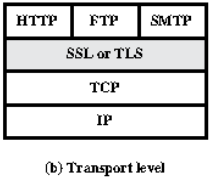
\includegraphics[width=0.4\linewidth]{chapters/10/images/intro.png}
\end{figure}

\noindent Vengono impiegati in ogni browser web, sistemi di pagamento, \dots

\section{SSL \textit{basics}}
SSL consiste in diversi protocolli:
\begin{itemize}
    \item \textbf{Handshake protocol:} usa chiave pubbliche per stabilire le chiavi 
    segrete condivise tra client e server 
    \item \textbf{Record protocol:} fornisce dei servizi di sicurezza ai protocolli di livello 
    più alto; usa le chiavi segrete per proteggere la confidenzialità, integrità e autenticità
    dei dati
    \item si \textit{negozia la versione del protocollo e gli algoritmi 
    crittografici da usare}
    \item \textit{autentica server e client} (opzionale); vengono usati dei certificati
    digitali per verificare le identità (spesso solo il server è autenticato)
\end{itemize}

\section{TLS \textit{basics}}
TLS si pone tra il livello applicativo e quello di trasporto: i dati non protetti 
vengono forniti a TLS, che li trasforma in dati criptati per poi fornirli al livello 
sottostante (trasporto).

\begin{figure}[H]
    \centering
    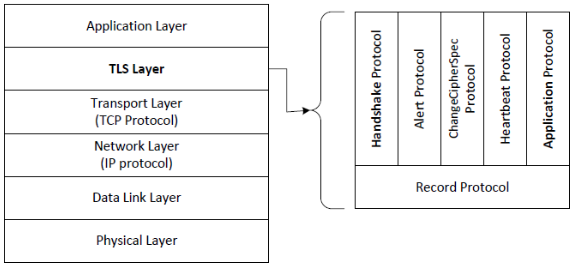
\includegraphics[width=1\linewidth]{chapters/10/images/tls-basics.png}
\end{figure}

\noindent In TLS ci sono \textit{due entità} principali:
\begin{itemize}
    \item \textbf{Connessione:} un trasporto che fornisce un tipo di servizio adeguate; in TLS, 
    tali connessioni sono relazioni \textit{peer-to-peer} (i nodi sono equivalenti)

    \noindent Ogni connessione è transitoria ed è associata ad una sessione
    \item \textbf{Sessione:} è un'associazione tra client e server creata dal protocollo di handshake;
    ogni sessione definise dei parametri crittografici di sicurezza che possono 
    essere condivisi tra più connessioni
    
    $\rightarrow$ vengono utilizzate per evitare la costosa negoziazione 
    di nuovi parametri di sicurezza per ogni connessione
\end{itemize}

\noindent Tra qualsiasi coppia di parti (ad esempio applicazioni come HTTP su client 
e server) potrebbero esserci più connessioni protette (in teoria anche più sessione,
ma non accade nella pratica).

\subsection{Componenti di TLS}

\subsubsection{Alert Protocol}
Notifica situazioni anomale o segnala eventuali problemi; viene usato per 
trasmettere allarmi relativi al protocollo SSL/TLS all'altra entità in 
comunicazione. Ogni messaggio è compsoto da \textbf{2 byte}:
\begin{itemize}
    \item il \textit{primo byte} assume il valore di \textbf{warning} o \textbf{fatal}
    che indica la gravità del messaggio identificato dal secondo byte; i messaggi \textit{fatal}
    sono irreversibili e la sessione viene interrota
    \item il \textit{secondo byte} contiene un codice che indica l'\textbf{avviso specifico}
\end{itemize}

\subsubsection{Handshake protocol}
Permette alle parti di negoziare i diversi algoritmi necessari per la sicurezza 
della comunicazione, consente l'eventuale autenticazione e lo scambio delle chiavi.

\noindent È fatto da una sequenza di messaggi, ciascuno dei quali ha i 
seguenti campi:
\begin{itemize}
    \item \textbf{Tipo} (1 byte): indica uno dei 10 tipi di messaggi disponibili
    \begin{itemize}
        \item \texttt{hello\_request}
        \item \texttt{client\_hello}
        \item \texttt{server\_hello}
        \item \texttt{certificate\_request}
        \item \texttt{certificate}
        \item \texttt{certificate\_verify}
        \item \texttt{server\_key\_exchange}
        \item \texttt{clinet\_key\_exchange}
        \item \texttt{server\_done}
        \item \texttt{finished}
    \end{itemize}
    \item \textbf{Lunghezza} (3 byte)
    \item \textbf{Contenuto} (byte): i parametri associati al messaggio
\end{itemize}

\begin{figure}[H]
    \centering
    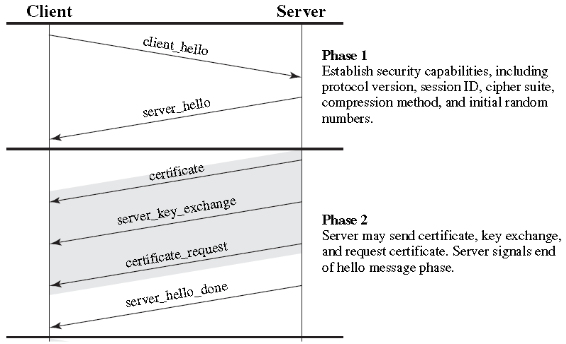
\includegraphics[width=1\linewidth]{chapters/10/images/hs1.png}
\end{figure}
\begin{figure}[H]
    \centering
    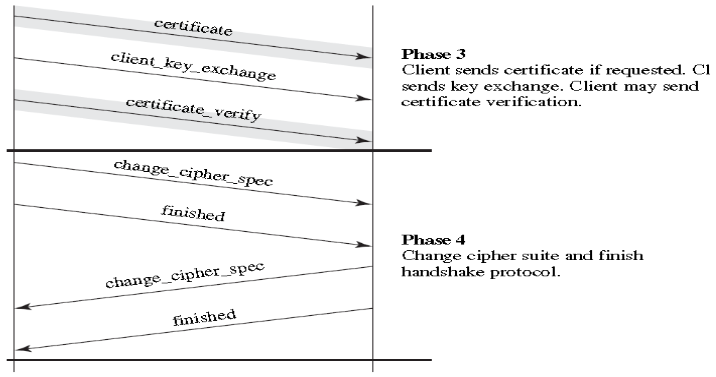
\includegraphics[width=1\linewidth]{chapters/10/images/hs2.png}
\end{figure}

\noindent La \textbf{generazione} e \textbf{scambio delle chiavi} viene fatta
in tre passaggi:
\begin{itemize}
    \item \textit{Segreto pre-master}: viene crittografato un numero casuale con la chiave pubblica del server 
    \item \textit{Segreto master}: viene generato usando i \textit{nonce} scambiati durante l'handshake e il 
    segreto pre-master 
    \item \textit{Chiave di sessione}: viene usato il segreto principale per generare 
    una sequenza di byte (le chiavi, dipendono dall'algortimo di cifratura)
\end{itemize}


\subsubsection{Change chiper spec protocol}
Impone l'esecuzione di un nuovo handshake per rinegoziare i parametri di sicurezza 
e ripetere l'autenticazione. 

\noindent È costituito da un singolo byte impostato al valore 1.

\subsubsection{Record protocol}
Fornisce \textit{due servizi} per le connessioni TLS:
\begin{itemize}
    \item \textbf{confidenzialità:} usa la chiave segreta condivisa durante l'handshake
    \item \textbf{integrità dei messaggi:} la stessa chiave segreta viene usata per il MAC (Message 
    Authentication Code)
\end{itemize}

I passagi che segue il protocollo sono:
\begin{enumerate}
    \item prende in input un messaggio da trasmettere 
    \item frammenta l'input in blocchi 
    \item applica il MAC al frammento (lo concatena in coda)
    \item cifra quanto ottenuto 
    \item aggiunge un'intestazione e trasmette in un segmento TCP; l'header contiene:
    \begin{itemize}
        \item \textit{content-type} (alert, handshake, \dots)
        \item \textit{versione}
        \item \textit{lunghezza del payload}
    \end{itemize}
\end{enumerate}

\begin{figure}[H]
    \centering
    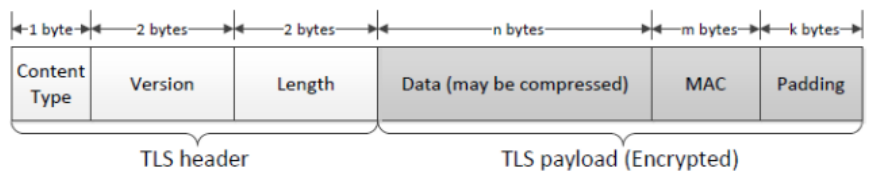
\includegraphics[width=1\linewidth]{chapters/10/images/tls-record.png}
\end{figure}

\subsection{Stato di sessioni e connessioni}

Lo stato di una sessione è definito da:
\begin{itemize}
    \item \textbf{identificatore}
    \item \textbf{certificato peer}
    \item \textbf{metodo di compressione} (da TLS 1.3 è vietato comprimere)
    \item \textbf{cipher spec:} algoritmo di crittografia usato e una funzione di hash da usare per il MAC 
    \item \textbf{master secret}
    \item \textbf{\texttt{isResumable}:} una flag che indica se è possibile avviare nuove connessioni dalla sessione
\end{itemize}

\noindent Lo stato di una connessione è definito da:
\begin{itemize}
    \item \textbf{server e client randomness} (sequenza di byte)
    \item \textbf{server write MAC secret}
    \item \textbf{client write MAC secret}
    \item \textbf{chiave di scrittura server}
    \item \textbf{chiave di scrittura client}
    \item \textbf{numeri di sequenza} 
\end{itemize}

\subsection{Costo di una sessione}
Sia lato client che lato server:
\begin{itemize}
    \item generare valori casuali 
    \item verifica dei certificati
    \item cifrare/decifrare i valori casuali con la chiave opportuna
    \item calcolare chiave con hash 
\end{itemize}

\noindent $\rightarrow$ ogni sessone ha un costo elevato; tanto richieste di connessione 
potrebbero portare ad un DoS

\section{SSH (Secure Shell)}
SSH è un protocollo di rete crittografico che permette di stabilire una sessione remota cifrata tramite interfaccia a riga di comando con un altro host di una rete informatica.

\noindent SSH è organizzato come tre protocolli che tipicamente vengono eseguiti su TCP:
\begin{itemize}
    \item \textbf{Transport Layer Protocol:} fornisce l'autenticazione del server, la riservatezza e l'integrità
    dei dati 
    \item \textbf{Protocollo di autenticazione utente} per autenticare l'utente sul server
    \item \textbf{Protocollo di connessione}
\end{itemize}

\noindent Sia TLS che SSH creano un tunnel per il trasporto di dati sicuro; hanno però alcune
differenze relative alla sua realizzazione, come i formati usati; inoltre, SSH ha dei protocolli 
per gestire ciò che accade all'interno del tunnel.


\section{Vulnerabilità}

\subsection{SSL \textit{version rollback}}
Il server viene ingannato pensando che sta comunicando con un client che 
supporta solo la versione SSL 2.0; questo è problematico perché:
\begin{itemize}
    \item le \textit{cipher spec} non sono autenticate 
    \item i messaggi dell'handshake non sono protetti 
    \item non supporta catene di certificazione
    \item \dots
\end{itemize}

\subsection{Man In The Middle TLS \textit{downgrade}}
Un utente malintenzionato che ha il controllo del traffico può simulare 
questo attacco ancora oggi.

Per gestire la connessione tra due dispositivi su una rete locale, bisogna 
fare in modo di reindirizzare il traffico attraverso l'attaccante, \textbf{manipolando 
la cache di ARP} (Address Resolution Protocol).

\section{HTTPS}
HTTPS è la versione sicura di HTTP; usa un canale sicuro SSL/TLS per inviare dei 
messaggi HTTP.

\noindent Bisogna fare attenzione che un attaccante non si introduca nel passaggio 
automatico tra HTTP e HTTPS: l'attaccante potrebbe redirizionare il traffico, 
intercettando i pacchetti della vittima e modificando la richiesta. 

\noindent La contromisura adottata è che le interazioni devono avvenire interamente 
in HTTPS; il browser si rifiuta di usare HTTP.

\section{Certificati}
I certificati in ambito web vengono rilasciati da un'ente accreditato a:
\begin{itemize}
    \item browser
    \item siti web
\end{itemize}

$\rightarrow$ prima di chiedere la pagina di un sito web, il browser richiede al web 
server il suo certificato; solamente dopo aver verificato chiede la pagina.

\noindent Un possibile attacco è quando un attaccante chiede un certificato legittimo
e ne crea una \textbf{copia falsa}, da usare ad esempio in un attacco di phishing.

\noindent Diventa fondamentale poter \textbf{revocare certificati}, ad esempio 
a causa di:
\begin{itemize}
    \item chiave privata compromessa 
    \item l'utente ha smesso di pagare per avere una certificazione, o non vuole più averla
    \item certificato compromesso
\end{itemize}


\chapter{Firewall}

\section{Introduzione ai firewall}

\subsubsection{Qualche nozione \dots}
\begin{itemize}
    \item \textbf{Minaccia:} causa di un incidente (\textit{perdita di 
    informazioni})
    \item \textbf{Vulnerabilità:} una debolezza di uno specifico sistema che può 
    rendere concreta una minaccia 
    \item \textbf{Attacco:} attuare una minaccia attraverso una vulnerabilità 
    \item \textbf{Vettore di attacco:} metodo o percorso attraverso il quale si concretizza 
    l'attacco (\textit{virus, email, \dots})
\end{itemize}

\noindent Lo scopo principale di un firewall è \textbf{controllare gli accessi}
da e per una rete protetta. Il controllo viene fatto obbligando le connessioni
a \textbf{passare attraverso il firewall}, dove vengono esaminate e valutate.

\noindent Bisogna ricordarsi che il firewall \textbf{non garantisce sicurezza 
assoluta}, poiché rimangono vulnerabili ad alcuni tipi di attacchi:
\begin{itemize}
    \item attacchi dall'interno della rete 
    \item non installare le security patch 
    \item errori di configurazione 
    \item mancanza di ispezioni approfondita dei pacchetti 
    \item attacchi DDoS non possono essere bloccati
\end{itemize}

\noindent I firewall hanno \textbf{tre principi inderogabili:}
\begin{enumerate}
    \item un firewall deve essere l'\textbf{unico punto di contatto} della rete interna con quella esterna 
    \item solo il \textbf{traffico autorizzato} può attraversare il firewall
    \item il firewall deve essere lui stesso un \textbf{sistema sicuro}
\end{enumerate}

\noindent Seguendo lo stack ISO/OSI, il firewall applica i seguenti controlli:
\begin{figure}[H]
    \centering
    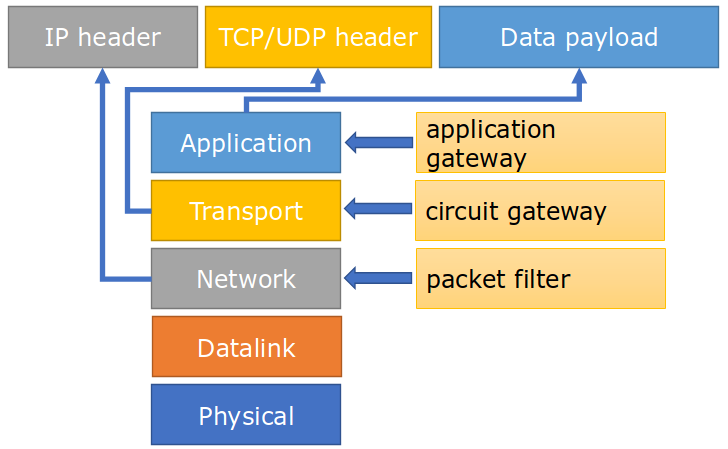
\includegraphics[width=0.8\linewidth]{chapters/11/images/controlli.png}
\end{figure}

\noindent Possiamo parlare di \textit{personal firewal} quando intendiamo una protezione 
orientata su un singolo host; è generalmente implementato come un filtro sw per 
proteggere il dispositivo da accessi indesiderati provenienti dall'esterno della rete.

\begin{figure}[H]
    \centering
    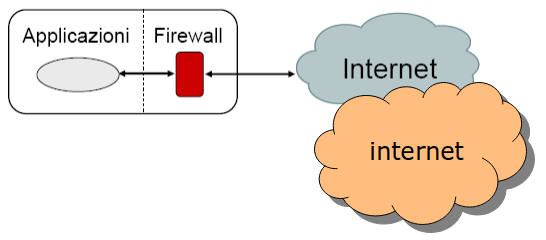
\includegraphics[width=0.6\linewidth]{chapters/11/images/personal-fw.png}
\end{figure}

\noindent Un \textit{firewall di rete} può anche essere una macchina dedicata che filtra tutto 
il traffico da e per una rete locale.

\begin{figure}[H]
    \centering
    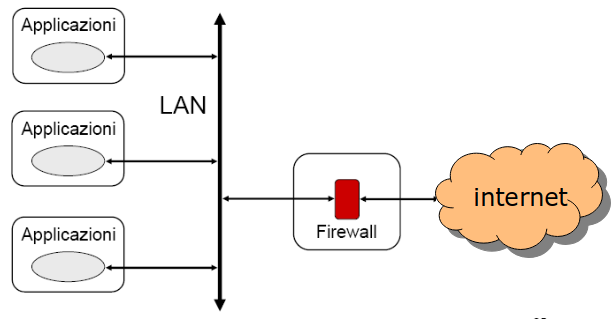
\includegraphics[width=0.6\linewidth]{chapters/11/images/fw.png}
\end{figure}


\subsection{Considerazioni architetturali}

Spesso i computer forniscono dei servizi che devono essere raggiungibili 
dall'esterno; allo stesso tempo, altri servizi devono essere protetti.
Per questa ragione la \textbf{rete protetta da un firewall viene divisa in due zone}:
\begin{itemize}
    \item \textbf{Rete pubblica:} è quel tratto di rete visibile da \textit{tutto il mondo}; ci possono essere situati
    un web server, mail server, \dots

    \noindent In gergo viene anche chiamata DMZ (\textit{de-militarized zone}), ovvero un tratto di rete in cui 
    il firewall permette l'accesso a tutti
    \item \textbf{Rete privata:} è la rete in cui i computer possono accedere ad internet ma non vengono
    visti dal \textit{mondo}
\end{itemize}

\begin{figure}[H]
    \centering
    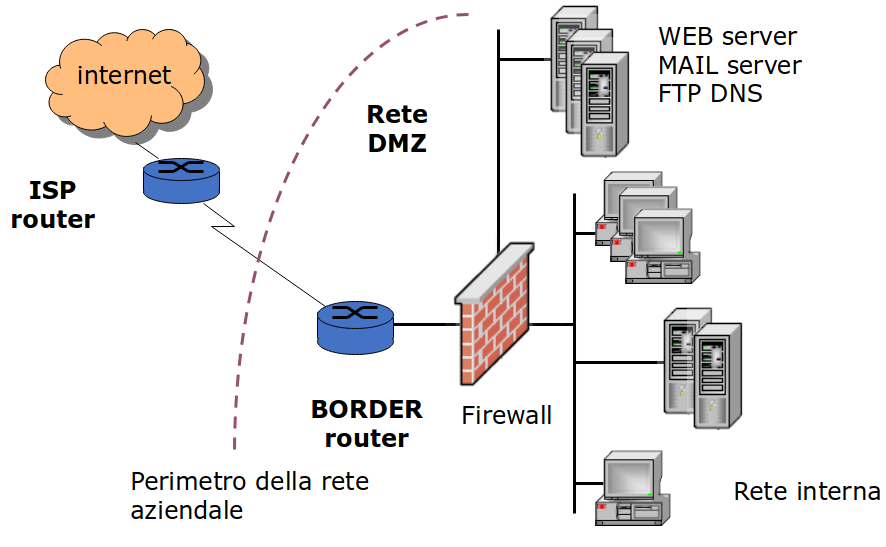
\includegraphics[width=1\linewidth]{chapters/11/images/zone.png}
\end{figure}

\noindent Sul firewall dovranno quindi essere installate tre \textit{interfacce di rete}:
\begin{itemize}
    \item una per il collegamento ad internet 
    \item una per la rete privata 
    \item una per la DMZ
\end{itemize}

\noindent Questa architettura prende il nome di \textbf{\textit{three-legged architecture}}.

\subsection{Protezione di rete}
\textbf{Tutto il traffico} tra la rete locale ed internet deve essere filtrato, mentre 
\textbf{solo il traffico autorizzato} può attraversare il firewall; i servizi 
necessari devono rimanere accessibili.

\noindent In fase di configurazione del firewall, si deve decidere la 
\textbf{politica di default} per i servizi di rete:
\begin{itemize}
    \item \textbf{\textit{Default deny:}} tutti i servizi non esplicitamente espressi sono negati 
    \item \textbf{\textit{Default allow:}} tutti i servizi non esplicitamente espressi sono permessi 
\end{itemize}

\noindent Il firewall permette di gestire una politica di accesso personalizzata per 
ogni sottorete ad esso collegata; solo i componenti esterni al firewall saranno 
senza protezione.

\noindent Si può inoltre gestire le connessioni tra le diverse interfacce del firewall 
(ad esempio, si può da internet alla DMZ ma non da internet alla rete privata).

$\rightarrow$ si può realizzare una separazione in zone aventi diverso grado di sicurezza 

\section{Packet Filtering}

\subsection{Static Stateless Packet Filtering (SPF)}
Il controllo del traffico è basato unicamente sulle informazioni contenute 
negli header dei singoli pacchetti.

\noindent I valori dei parametri degli header dei pacchetti vengono \textbf{confrontati 
con le regole definite in una ACL} (\textit{Access Control List}) e ammessi o scartati 
secondo il risultato del confronto.

$\rightarrow$ ogni pacchetto viene esaminato singolarmente, \textbf{indipendemente dagli altri pacchetti} precedenti 
o successivi

\noindent Il filtro scarta i datagrammi IP sulla base di:
\begin{itemize}
    \item tipo di servizio a cui il datagramma è destinato (porta TCP/UDP)
    \item indirizzo IP sorgente/destinazione 
    \item indirizzo MAC sorgente/destinazione 
    \item interfaccia di provenienza/destinazione 
\end{itemize}

\noindent Questa è la prima e più semplice tecnologia adottata per i sistemi di 
firewall. Nei sistemi odierni è stata superata dalla tecnologia di tipo \textit{stateful}, ma continua
ad essere usata nei sistemi di fascia bassa e nei router per la sua semplicità e per 
le ottime performance

\noindent Dato che \textit{Static} e \textit{Stateless} vanno di norma assieme, questo tipo di firewall
si può semplificare con \textbf{Static Packet Filter (SPF)}.

\subsection{Applicazioni di SPF}
Spesso, per alcuni servizi, si impone che le comunicazioni vengano regolate in 
modo tale che dalla rete interna si possa raggiungere l'esterno, ma non il contrario (ad esempio ping, SSH, \dots).

\subsubsection{Connessioni TCP}
Durante l'handshake, attraverso i FLAG dell'header TCP possiamo supportare la politica 
di sicurezza (ad esempio, solo da dentro a fuori).

\begin{figure}[H]
    \centering
    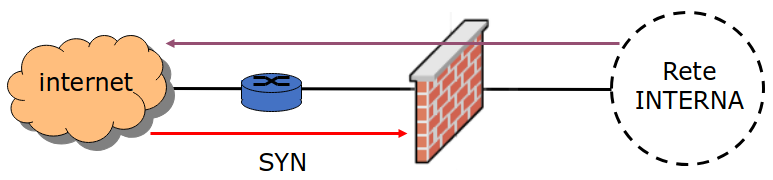
\includegraphics[width=0.8\linewidth]{chapters/11/images/spt-tcp.png}
\end{figure}

\subsection{Efficacia}
STP è capace di proteggere da:
\begin{itemize}
    \item attacchi elementari di \textbf{spoofing}
    \item \textbf{tentate connessioni}, tramite controllo degli IP, porte di destinazione e flag TCP 
    \item \textbf{traffico ICMP malevolo}
\end{itemize}

\noindent $\rightarrow$ è utile se configurato su un router come primo livello di protezione perimetrale; protegge solo da 
tecniche di attacco non sofisticate

\subsection{Stateful Filtering}
Un packet filter può essere \textit{stateless} o \textit{stateful}. Questa separazione 
ormai è più teorica che pratica, dato che tutte le implementazioni di SPF offrono anche qualche tipo 
di \textit{protocol inspection}, per cui sono \textbf{multilayer stateful firewall}.

\subsubsection{Protocol inspection}
La \textbf{stateful} inspection è quel processo per cui ogni singola connessione autorizzata 
viene registrata dal firewall in una apposita tabella, la cosidetta \textbf{connection} o \textbf{state table}:
\begin{itemize}
    \item oltre all'IP sorgente e di destinazione, vengono registrati tanti altri dati, come 
    il protocollo, le porte, i flag, sequence number \dots
\end{itemize}

$\rightarrow$ è difficile per un hacker inserirsi in una connessione stabilita (\textit{session hijacking})

\noindent Nella pratica, ogni volta che un pacchetto arriva al firewall, viene verificato 
se esso fa parte di una connessione precedentemente stabilita:
\begin{itemize}
    \item in caso affermativo, viene lasciato passare senza ulteriori controlli 
    \item altrimenti subisce i controlli di un normale pacchetto in ingresso
\end{itemize}

\subsection{Considerazioni sul packet filtering}
Anche con la migliore configurazione il packet filter \textbf{non verifica 
il contenuto dei pacchetti}, per cui non può bloccare virus; inoltre, ha problemi
con i protocolli che allocano le porte in maniera dinamica come FTP.

\section{Access Control List}
Le ACL definiscono regole per il filtraggio statico dei pacchetti in transito. La semantica 
è ACCEPT/DENY, ed utilizzano un criterio \textit{top-down} di filtraggio:
\begin{itemize}
    \item la prima regola che viene verificata produce la decisione sul pacchetto
    \item il test del pacchetto continua fino a che una regola corrisponde alle caratteristiche 
    del pacchetto oppure fino a che la lista di regole termina 
    \item di norma esiste una regola di default
    \begin{itemize}
        \item Default Permit 
        \item Default Deny 
    \end{itemize}
\end{itemize}

\noindent Le ACL lavorano al livello \textit{network} della pila ISO/OSI.

\subsection{Standard ACL}
Le \textit{standard ACL} sono numerate tra 0 e 99, filtrano \textbf{solo} gli 
indirizzi \textbf{IP sorgente}.

\begin{center}
    \texttt{Access-list numero azione sorgente [wild card] | any}
\end{center}

\begin{itemize}
    \item Numero: da 0 a 99 
    \item Azione: \textit{permit} o \textit{deny}
    \item Sorgente: indirizzo IP sorgente 
    \item Wild card: determina la parte dell'indirizzo IP da verificare e quella di ignorare;
    è simile alla netmask, ma ha una semantica dei valori invertita:
    \begin{itemize}
        \item valore binario 1: bit dell'indirizzo IP non deve essere verificato
        \item valore binario 0: bit dell'indirizzo IP deve essere verificato 
    \end{itemize}
    \item Any: qualunque valore
\end{itemize}

\subsubsection{Esempi}
\begin{itemize}
    \item \texttt{Access-list 17 permit host 192.168.1.100}
    \begin{itemize}
        \item la keyword \texttt{host} si usa quando si indica un indirizzo IP unico; analogo 
        ad usare wildcard 0.0.0.0
    \end{itemize}
    \item \texttt{Access-list 17 deny 192.168.1.0 0.0.0.255}
    \item \texttt{Access-list 17 permit any}
    \begin{itemize}
        \item la regola di default viene fatta usando \texttt{permit any} oppure \texttt{deny any}
    \end{itemize}
\end{itemize}

\noindent Le ACL possono essere categorizzate in due:
\begin{itemize}
    \item \textbf{Ingress firewall:} controllo sui collegamenti \textit{incoming}, tipicamente verso 
    servizi offerti all'esterno
    \item \textbf{Egress firewall:} controllo sui collegamenti \textit{outgoing}; controllo sull'attività del personale
\end{itemize}

\noindent Questa distinzione è facile per i servizi orientati al canale (TCP), più difficile 
per quelli basati su datagrammi (UDP, ICMP).

\subsection{Extended ACL}
\begin{center}
    \texttt{Access-list numero azione tipo sorgente [wild card] opzioni
    destinazione [wild card] [log]}
\end{center}

\begin{itemize}
    \item Numero: da 100 a 199 
    \item Azione: Permit/Deny
    \item Tipo: IP, UDP o TCP 
    \item Sorgente: indirizzo IP sorgente 
    \item Opzioni: porte TCP/UDP, Tipo/Codice ICMP, operatori speciali:
    \begin{itemize}
        \item eq: \textit{equal} 
        \item neq: \textit{not equal}
        \item gt: \textit{greater than} 
        \item lt: \textit{less than}
    \end{itemize}
    \item Log: scrive un messaggio in un log per ogni pacchetto verificato da una regola
\end{itemize}

\subsubsection{Esempi}
\begin{itemize}
    \item \texttt{Access-list 101 permit tcp 192.168.2.0 0.0.0.255 any eq 23}
    \item \texttt{Access-list 101 permit tcp 192.168.2.0 0.0.0.255 any eq ftp}
\end{itemize}

\noindent Come si può vedere, gli operatori logici possono essere usati sia con numeri di 
porta che con keyword. 

\noindent È possibile usare \texttt{eq established} per accettare unicamente delle 
connessioni TCP già stabilite.

\subsection{ACL e interfacce}
Una volta definita una ACL, è necessario \textbf{associarla ad un'interfaccia}
del dispositivo di rete:

\begin{center}
    \texttt{ip access-group accessListNumber \{in|out\}}
\end{center}

\begin{itemize}
    \item accessListNumber: indica il numero dell'ACL che deve essere legata all'interfaccia 
    \item in|out: specifica se l'ACL vada applicata al traffico in entrata o in uscita
\end{itemize}

\section{ACL e protocolli applicativi}

\subsection{Esempio}
Si vuole negare all'host B l'accesso al Server FTP e allo stesso tempo negare all'host C 
qualsiasi accesso alla rete 172.16.3.0

\begin{figure}[H]
    \centering
    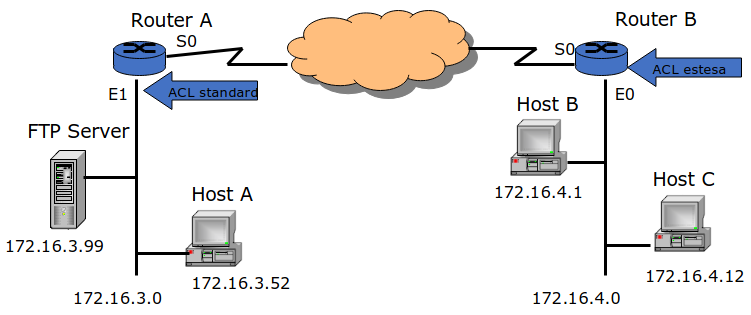
\includegraphics[width=1\linewidth]{chapters/11/images/esempio.png}
\end{figure}

\begin{lstlisting}
    access-list 1 deny host 172.16.4.12 
    access-list 1 permit any
    interface ethernet 1 (E1)
    ip access-group 1
    access-list 101 deny tcp host 172.16.4.1 172.16.3.0 0.0.0.255 eq ftp 
    access-list 101 permit ip 172.16.4.0 0.0.0.255 any 
    interface ethernet 0 (E0)
    ip access-group 101
\end{lstlisting}

\subsection{Formalismo}
Una ACL Static Packet Filter è definita da una tabella come la seguente:

\begin{figure}[H]
    \centering
    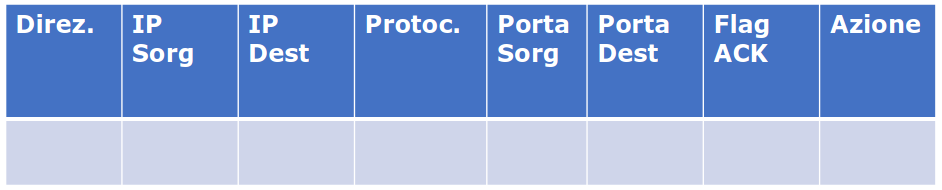
\includegraphics[width=1\linewidth]{chapters/11/images/tabella.png}
\end{figure}

\noindent È molto diffuso l'uso di variabili alle quali assegnare dei parametri, tipicamente indirizzi IP e sottoreti. L'utilizzo delle variabili 
al posto dei valori permette di:
\begin{itemize}
    \item separare la definizione dei valori dalle definizione della politica del firewall
    \item si possono modificare i valori senza modificare la politica stessa
\end{itemize}

\subsection{Esempio con Telnet}
Vogliamo autorizzare solo connessioni Telnet (assegnato alla porta 23) dall'interno della rete aziendale verso 
l'esterno.

\begin{figure}[H]
    \centering
    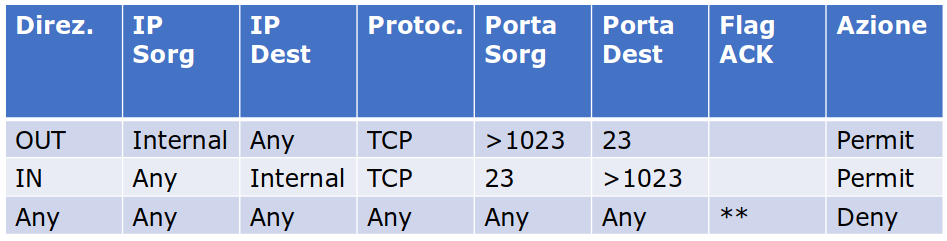
\includegraphics[width=1\linewidth]{chapters/11/images/telnet1.png}
\end{figure}

\noindent Filtrare il traffico solo sulle porte sorgente e destianzione può 
portare ad una politica troppo permissiva. Ad esempio, la regola 

\begin{center}
    \texttt{IN any Internal TCP 23 >1023 Permit} 
\end{center}

\noindent permette connessioni generate da qualunque host esterno e dirette a qualunque host interno 
aventi porta sorgente 23/TCP e porta destinataria $>1023$

\newpage Sappiamo che i pacchetti provenienti dall'esterno della rete sono solo
le risposte del server. Possiamo limitare la politica ai soli server utilizzati:

\begin{figure}[H]
    \centering
    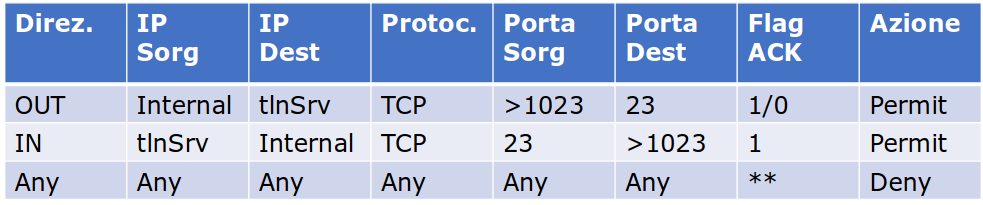
\includegraphics[width=1\linewidth]{chapters/11/images/telnet2.png}
\end{figure}

\noindent Usiamo ACK:
\begin{itemize}
    \item 1/0 quando IP sorgente stabilisce la connessione verso IP destinatario 
    \item 1 quanod IP sorgente risponde all'IP destinatario
\end{itemize}


\noindent In generale, \textbf{la politica di un firewall deve essere la più stringente 
possibile; è un errore definire una politica più \textit{lasca} dello stretto necessario}.



\chapter{Firewall Avanzati}

Applicazioni come Telnet, SSH, rlogin \dots sono semplici da gestire con 
packet filtering, perché per loro natura implicano ruoli ben definiti: client 
e server; il pattern di scambio è un semplice request/reply.

Altre applicazioni possono avere protocolli più elaborati; quando lo 
scambio a livello di trasporto diventa più articolato, gestire il firewall 
diventa più complesso:
\begin{itemize}
    \item studiare molto bene i protocolli applicativi 
    \item verificare debolezze del filtraggio 
    \item essere consapevoli di cosa non si riesce a fare con il filtraggio 
\end{itemize}

\section{Packet Filtering Avanzati}

\subsection{SMTP (Simple Mail Transfer Protocol)}
Gestisce lo scambio di messaggi di posta elettronica:
\begin{itemize}
    \item la connessione tra i diversi server di posta avviene attraverso una connessione 
    TCP (porta 25)
    \item Ogni utente è identificato dall'indirizzo \textit{nomeutente@indirizzo\_server}
\end{itemize}

\noindent Il client a livello utente utilizza SMTP solo per inviare il messaggio al 
server mail, il quale poi lo invierà \textit{"davvero"}.

\subsubsection{I comandi}
I principali comandi SMTP:
\begin{itemize}
    \item \textbf{HELO}: identifica il client SMTP al server SMTP
    \item \textbf{EHLO}: possibile usare anche questo comando per identificarsi, se supportato dal server
    \item \textbf{MAIL FROM $<$indirizzo mittente$>$}: indica mailbox del mittente 
    \item \textbf{RCPT TO $<$indirizzo destinatario$>$}: mailbox destinatario; è possibile 
    indicare molteplici destinatari 
    \item \textbf{DATA}: indica al server che quanto digitato successivamente sono i dati del messaggio di posta
    \item \textbf{RSET}: annulla i comandi precedentemente inviati nella sessione corrente 
    \item \textbf{VRFY $<$stringa$>$}: chiede al server se la stringa rappresenta un nome utente, ed in tal 
    caso visualizza il suo indirizzo 
    \item \textbf{HELP}: visualizza i comandi disponibili sul server 
    \item \textbf{NOOP}: non esegue alcuna operazione, restituisce un messaggio 250 (OK) se il server risponde 
    \item \textbf{QUIT}: termina la sessione corrente
\end{itemize}

\subsubsection{Le fasi}
Una sessione SMTP attraversa almeno sei fasi:
\begin{enumerate}
    \item Il client SMTP contatta il server sulla porta 25; se è in ascolto e 
    la connessione è accettata risponde con un messaggio 220 (\textit{Ready})
    \item Il client chiede di stabilire la connessione inviando il comando HELO seguito 
    dal FQDN (Fully Qualified Domain Name); se il server accetta risponde con 250 (OK)
    \item Il client indica il proprio indirizzo tramite il comando MAIL FROM; il server risponde 250 (OK)
    \item Il client indica i destinatari tramite RCPT TO; il server risponde 250 (OK) per ogni destinatario accettato 
    \item Il client comunica l'intenzione di scrivere il corpo del messaggio con DATA
    \item Completato il messaggio il server memorizza la mail; è possibile scrivere un nuovo messaggio 
    oppure inviare il comando QUIT, dopo il quale il server invia i messaggi e risponde con Closing (221); la 
    connessione TCP viene terminata
\end{enumerate}

\subsubsection{I codici di risposta}
Il server risponde ad ogni comando con un codice di tre cifre che ha la 
seguente interpretazione:
\begin{itemize}
    \item 1xx: messaggio informativo
    \item 2xx: comando eseguito e terminato con successo 
    \item 3xx: comando eseguito e terminato con successo che richiede di essere 
    seguito da altri comandi 
    \item 4xx: errore temporaneo nell'esecuzione del comando, ma il dialogo non è compromesso 
    \item 5xx: errore grave, il dialogo è compromesso e dovrà essere ripreso dall'inizio
\end{itemize}

\subsubsection{Protezione}
\begin{itemize}
    \item Protezione anti-spam minimale
    \begin{itemize}
        \item verifica del dominio del mittente 
        \item login obbligatorio
        
        $\rightarrow$ fatto per evitare \textbf{\textit{open relay}}, ovvero la capacità di mandare posta 
        senza essere autenticato 
    \end{itemize}
    \item Si aggiunge la criptazione al servizio di posta (con SSL/TLS); così viene criptata 
    il \textit{canale} ma non il messaggio, quindi un server intermediario può leggere 

    $\rightarrow$ se voglio criptare anche il messaggio si usa un altro protocollo (PGP)
\end{itemize}

\subsubsection{Packet Filtering}
\begin{itemize}
    \item \textbf{Politica:} nella rete aziendale un solo server SMTP è autorizzato 
    a gestire la posta elettronica con l'esterno 
    
    $\rightarrow$ bisogna gestire due connessioni TCP:
    \begin{itemize}
        \item Ricevere posta elettronica: altri mail server si connettono al mail server aziendale agendo da client 
        \item Inviare posta elettronica: il mail server aziendale si connette ad altri mail server agendo da client
    \end{itemize}
\end{itemize}

\begin{figure}[H]
    \centering
    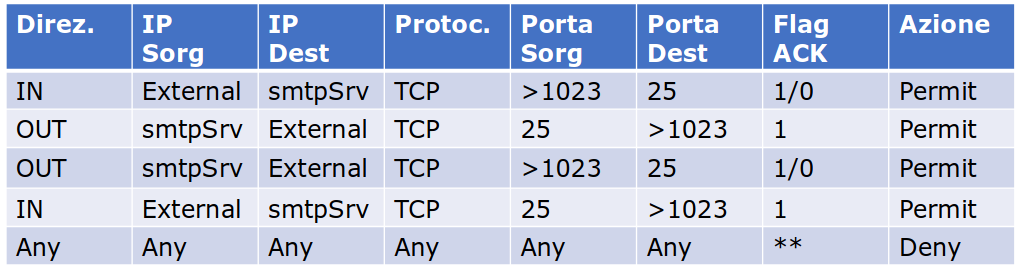
\includegraphics[width=1\linewidth]{chapters/12/images/smtp.png}
\end{figure}

\subsection{FTP (File Transfer Protocol)}
FTP è il protocollo generalmente usato per trasferire dati tra due host, con l'obiettivo 
di farlo in maniera efficiente ed affidabile; per questo motivo si basa su TCP (porta 21).

\noindent FTP utilizza due processi distinti:
\begin{itemize}
    \item \textit{Protocol Interpreter} (PI) attraverso cui il client invia comandi e riceve le risposte del server 
    \item \textit{Data Transfer Process} (DTP) attraverso cui il client ed il server si scambiano dati;
    può essere di due tipi:
    \begin{itemize}
        \item Attivo: il client contatta il server il quale da inizio alla connessione 
        \item Passivo: è prerorgativa del client anche dare il via alla connessione
    \end{itemize}
\end{itemize}

\subsubsection{Le fasi}
\begin{enumerate}
    \item Il client contatta il server sulla porta 21 usando il PI
    \item Autenticazione del client 
    \item Trasferimento dati tramite DTP 
    \item Termine della sessione TCP 
\end{enumerate}

\subsubsection{Connessioni FTP}
Ci sono due connessioni TCP per ogni sessione FTP:
\begin{itemize}
    \item \textbf{Connessione di controllo:} usata dal client per inviare i comandi e 
    dal server per comunicare i codici di risposta; viene aperta dal client che si connette 
    al server sulla porta TCP 21 
    \item \textbf{Connessione dati:} usata per il trasferimento dei file, viene aperta 
    dal server sulla porta 20
\end{itemize} 

\noindent La connessione dati viene aperta dal server verso il client:
\begin{center}
    \texttt{ftpServer:20} $\rightarrow$ \texttt{ftpClient:XXXX}
\end{center}

\noindent dove XXXX è la porta definita dinamicamente dal client.

\noindent $\rightarrow$ Non è possibile applicare la solita politica di gestione, dato che 
la connessione da esterno ad interno è obbligata ma non sappiamo a priori la porta.

\noindent Rischio:
\begin{center}
    \texttt{Intusore:20} $\rightarrow$ \texttt{Vittima:XXXX}
\end{center}

\noindent Le porte $>$1023 sono usate da servizi molto diffusi e da trojan.

\begin{figure}[H]
    \centering
    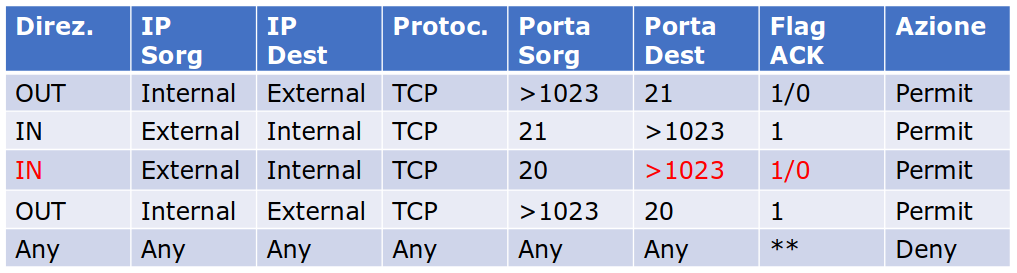
\includegraphics[width=1\linewidth]{chapters/12/images/ftp1.png}
\end{figure}

\noindent Dovrei usare un packet filtering che si ricordi delle connessioni.
\subsubsection{Soluzione}
La connessione dati viene aperta dal client verso il server (DTP passivo).

\begin{center}
    \texttt{ftpClient:YYYY} $\rightarrow$ \texttt{ftpServer:XXXX}
\end{center}

La politica di gestione \textit{connessioni solo da interno ad esterno} torna 
ad essere applicabile. Ora tutti gli FTP supportano la modalità passiva di default.

\begin{figure}[H]
    \centering
    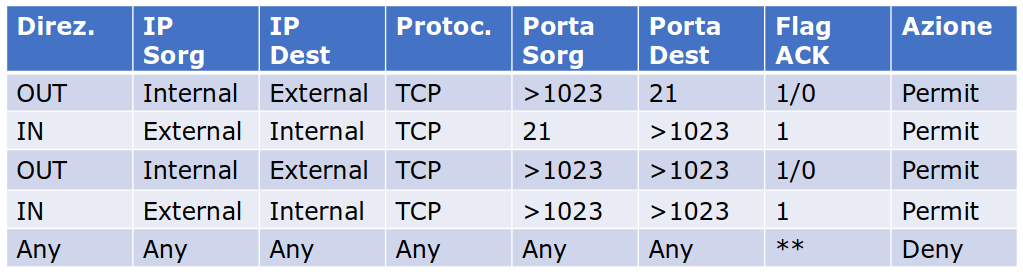
\includegraphics[width=1\linewidth]{chapters/12/images/ftp2.png}
\end{figure}

\subsection{Attacco RPC}
Remote Call Procedure è un protocollo che può essere utilizzato 
da un'applicazione per richiedere un serivizio a un programma residente su un 
altro computer in rete. 
\noindent È stata riscontrata una vulnerabilità che potrebbe portare all'esecuzione 
di codice non autorizzato.

\noindent A livello di firewall il problema è che non si conosce a priori la
porta che il server RPC assegnerà al servizio. Rischio:
\begin{center}
    \texttt{Intrusore:YYYY} $\rightarrow$ \texttt{ServerRPC-Vittima:XXXX}
\end{center}

\section{New Generation Packet Filtering}

Lo svantaggio principale dell'approccio SPF risiede nell'\textbf{array di porte 
che devono essere lasciate aperte} per tutto il tempo per permettere il 
traffico desiderato.

\subsubsection{Dynamic Packet Filter}

\noindent Per superare questo problema sono stati sviluppati dei \textbf{Dynamic Packet Filter},
che aprono e chiudono le porte sul firewall in base alle info dell'header dei 
pacchetti che transitano attraverso di essi; una volta che una serie di pacchetti 
ha transitato attraverso la porta, il firewall richiude la porta.

\subsubsection{Stateful Packet Filter}
È una evoluzione del dynamic ma \textit{state-aware}:
\begin{itemize}
    \item prende informazioni dai livelli superiori (trasporto e/o applicativo) per cercare di adattare 
    di conseguenza le regole di filtraggio 
    \item distingue le nuove connessioni da quelle già apert, tenendo traccia delle sessioni
\end{itemize}

\subsection{Vantaggi e Svantaggi del Dynamic Packet Filter}
\begin{itemize}
    \item \textbf{\textcolor{darkgreen}{Vantaggi:}}
    \begin{itemize}
        \item le porte sono aperte solo temporaneamente sul perimetro della rete 
        \item supporta quasi tutti i servizi 
        \item molti attacchi che funzionano su SPF sono difficili o impossibili da replicare 
        su DPF
    \end{itemize}
    \item \textbf{\textcolor{red}{Svantaggi:}}
    \begin{itemize}
        \item permettono connessioni IP dirette verso gli host interni della rete
        \item non garantiscono alcuna autenticazione
        \item soggetto ad attacchi che mirano alla saturazione della tabella  
    \end{itemize}
\end{itemize}

\subsection{Connessioni TCP - stateful firewall}
\begin{itemize}
    \item Alla ricezioni di un SYN $\rightarrow$ verifica dell'ACL
    \begin{itemize}
        \item connessione non autorizzata $\rightarrow$ deny 
        \item connessione autorizzata $\rightarrow$ accept e scrittura di una entry nella connection table 
    \end{itemize}
    \item Ricezione di pacchetti successivi $\rightarrow$ verifica della connection table
\end{itemize}

\noindent $\rightarrow$ è necessario definire solo le regole relative all'apertura delle 
connessioni TCP (pacchetto SYN)

\subsection{UDP - stateful firewall}
UDP non ha uno stato della connessione per definizione; viene impostato dunque un \textbf{timeout}
verificando anche chi ha impostato la connessione per primo.
\noindent Molti sistemi stateful hanno la possibilità di fare filtraggio applicativo:
\begin{itemize}
    \item comporta che il firewall faccia il parsing del pacchetto e conosca i protocolli 
    \item tutto ciò a scapito delle performance
\end{itemize}

\subsection{Deep Packet Inspection}
Il controllo non viene fatto solo sul protocollo ma anche sul pattern di comunicazione usato. Ad 
esempio, le richieste che rispettano il protocollo ma sono tipicamente usate per un attacco vengono respinte.
\begin{itemize}
    \item offre una protezione migliore
    \item definizione più semplice della politica 
    \item impatta pesantemente sulle prestazioni
\end{itemize}




\chapter{IDS (Intrusion Detection System)}

Dato che i firewall non possono proteggere da tutte le minacce e un \textit{instrusione}
non è un evento impossibile, è fondamentale e rilevarla e porre rimedio; viene 
fatto tramite gli \textbf{Intrusione Detection Systems}:
\begin{itemize}
    \item \textbf{sistema per identificare individui/servizi che usano un computer o una 
    rete senza autorizzazione}; il controllo è esteso anche ad utenti autorizzati, ma 
    che \textbf{non rispettano i loro privilegi}
    \item viene fatto monitorando il traffico di rete; può collaborare con il firewall
    \item è utile anche per fornire informazioni utili su intrusioni avvenute, fare diagnosi e correggere debolezze
\end{itemize} 

\noindent È importante ricordare che gl'IDS \textbf{non è un sistema di protezione 
ma di rilevazione} delle intrusioni o di attacchi provenienti dall'esterno.

\subsubsection{Caratteristiche funzionali}
\begin{itemize}
    \item \textbf{IDS passivi:}
    \begin{itemize}
        \item checksum crittografici 
        \item riconoscimento di pattern 
    \end{itemize}
    \item \textbf{IDS attivi:}
    \begin{itemize}
        \item \textit{learning} $\rightarrow$ analisi statistica del sistema 
        \item \textit{monitoring} $\rightarrow$ analisi attiva del traffico di dati, azionim \dots
        \item \textit{reaction} $\rightarrow$ confronto con parametri statistici (reazione scatta al superamento di una soglia)
    \end{itemize}
\end{itemize}

\section{Caratteristiche topologiche}

\begin{itemize}
    \item \textbf{HIDS (host-based IDS):}
    \begin{itemize}
        \item analisi dei log 
        \item attivazione di strumenti di monitoraggio interni al S.O.
    \end{itemize}
    \item \textbf{NIDS (network-based IDS):}
    \begin{itemize}
        \item attivazione di strumenti di monitoraggio del traffico di rete 
    \end{itemize}
\end{itemize}

\subsubsection{Componenti di un NIDS}
\begin{itemize}
    \item \textbf{Sensor:} controlla il traffico e log per individuare pattern sospetti; attiva i 
    security event quando necessario
    \item \textbf{Director:} coordina i sensor 
    \item \textbf{IDS message system:} consente la comunicazione sicura tra i componenti dell'IDS
\end{itemize}



\section{Valutare un IDS}
Per valutare l'efficienza di un IDS occorre conoscere due parametri:
\begin{itemize}
    \item \textbf{Accuratezza:} $allarmi Corretti / allarmi Totali$
    \item \textbf{Completezza:} $allarmi Corretti / intrusioni Totali$
\end{itemize}

\noindent Occore sempre bilanciare i \textit{falsi negativi}
e i \textit{falsi positivi}, dato che questi parametri sono correlati inversamente.














\end{document}